%%%%%%%%%%% Aquí va la solución al problema 4.
\newpage
\textbf{\textcolor{MidnightBlue}{4.}} Considera el algoritmo 1,
que calcula una $\Delta + 1$ coloración, donde $\Delta$ es el
grado máximo en la gráfica. Muestra una gráfica $G$ con al menos
10 vértices y una asignación de IDs, donde el algoritmo coloree
todos los procesos (el primer momento en el que todas las variables
$c$ son distintas de $\bot$) en tiempo $diam(G)$. Muestra otra
asignación de IDs para las que el algoritmo coloree en tiempo a los
más $diam(G)/2$.

\begin{figure}[ht]
        \begin{center}
                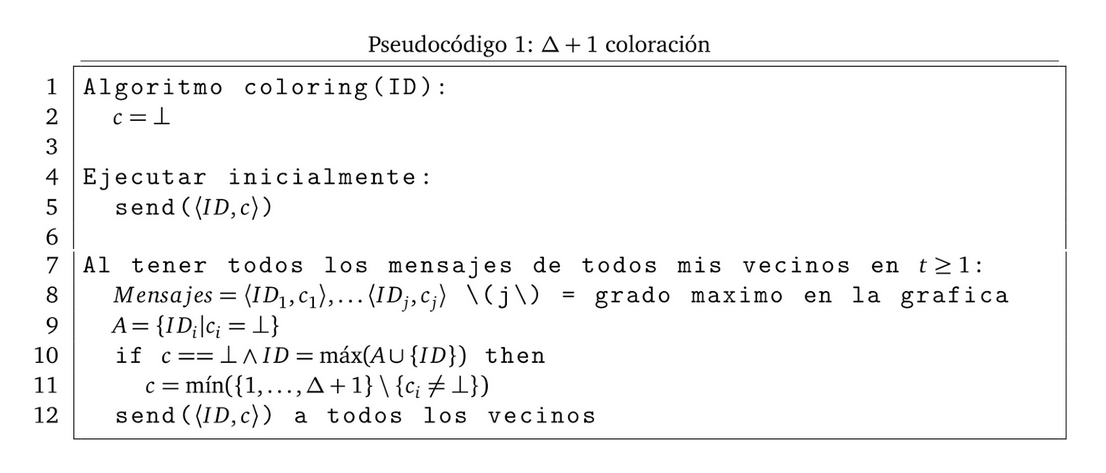
\includegraphics[width=15cm]{AlgoritmoP5.png}
        \end{center}
\end{figure}

$\rhd$ Para este problema dividamos la solución en $2$ respectivas
soluciones:                                                             \newline

\hspace*{0.5cm} \textbf{\textcolor{blue}{1}}. Mostrar una ejecución
en tiempo $\code{diam($G$)}$, con $G$ una gráfica tal que $|V_G| = 10$.

\begin{figure}[ht!]
     \centering
     \begin{tikzpicture}
        \begin{scope}
           % Fig exterior:
           \node(0) [vertex, label=180:$p_8$] at (0, 6)        {};
           \node(1) [vertex, label=360:$p_2$] at (3.24, 3.81)  {};
           \node(2) [vertex, label=360:$p_3$] at (2,  0)       {};
           \node(3) [vertex, label=180:$p_4$] at (-2, 0)       {};
           \node(4) [vertex, label=180:$p_5$] at (-3.24, 3.81) {};
           % Fig interior:
           \node(5) [vertex, label=180:$p_6$] at (0, 4.5)      {};
           \node(6) [vertex, label=180:$p_1$] at (1.6,  3.4)   {};
           \node(7) [vertex, label=180:$p_0$] at (1, 1.5)      {};
           \node(8) [vertex, label=180:$p_7$] at (-1, 1.5)     {};
           \node(9) [vertex, label=180:$p_9$] at (-1.6, 3.4)   {};
           
           % Segmentos
           \draw [edge] (1) to (2);
           \draw [edge] (2) to (3);
           \draw [edge] (3) to (4);
           \draw [edge] (4) to (0);
           \draw [edge] (0) to (5);
           \draw [edge] (1) to (6);
           \draw [edge] (5) to (8);
           \draw [edge] (6) to (7);
           \draw [edge] (9) to (8);
           
           \node (L) at (-3,6){$G$};
        \end{scope}
     \end{tikzpicture}
\caption{Gŕagica $G$.}
\label{fig:fam1}
\end{figure}

En la ronda 0 tenemos que: \newline

Se envían los $ID_i$'s a todos los vecinos para cada proceso, por
motivos de visualización de la gráfica no se ilustra cada $ID_i$
para algún $i \in [0, \dotsm, 9]$, pero cuándo sea necesario se
indicara \footnote{Además es claro que para un proceso $p_j$ existe
un $ID_j$ único.}. \newpage

\begin{figure}[ht]
        \begin{center}
                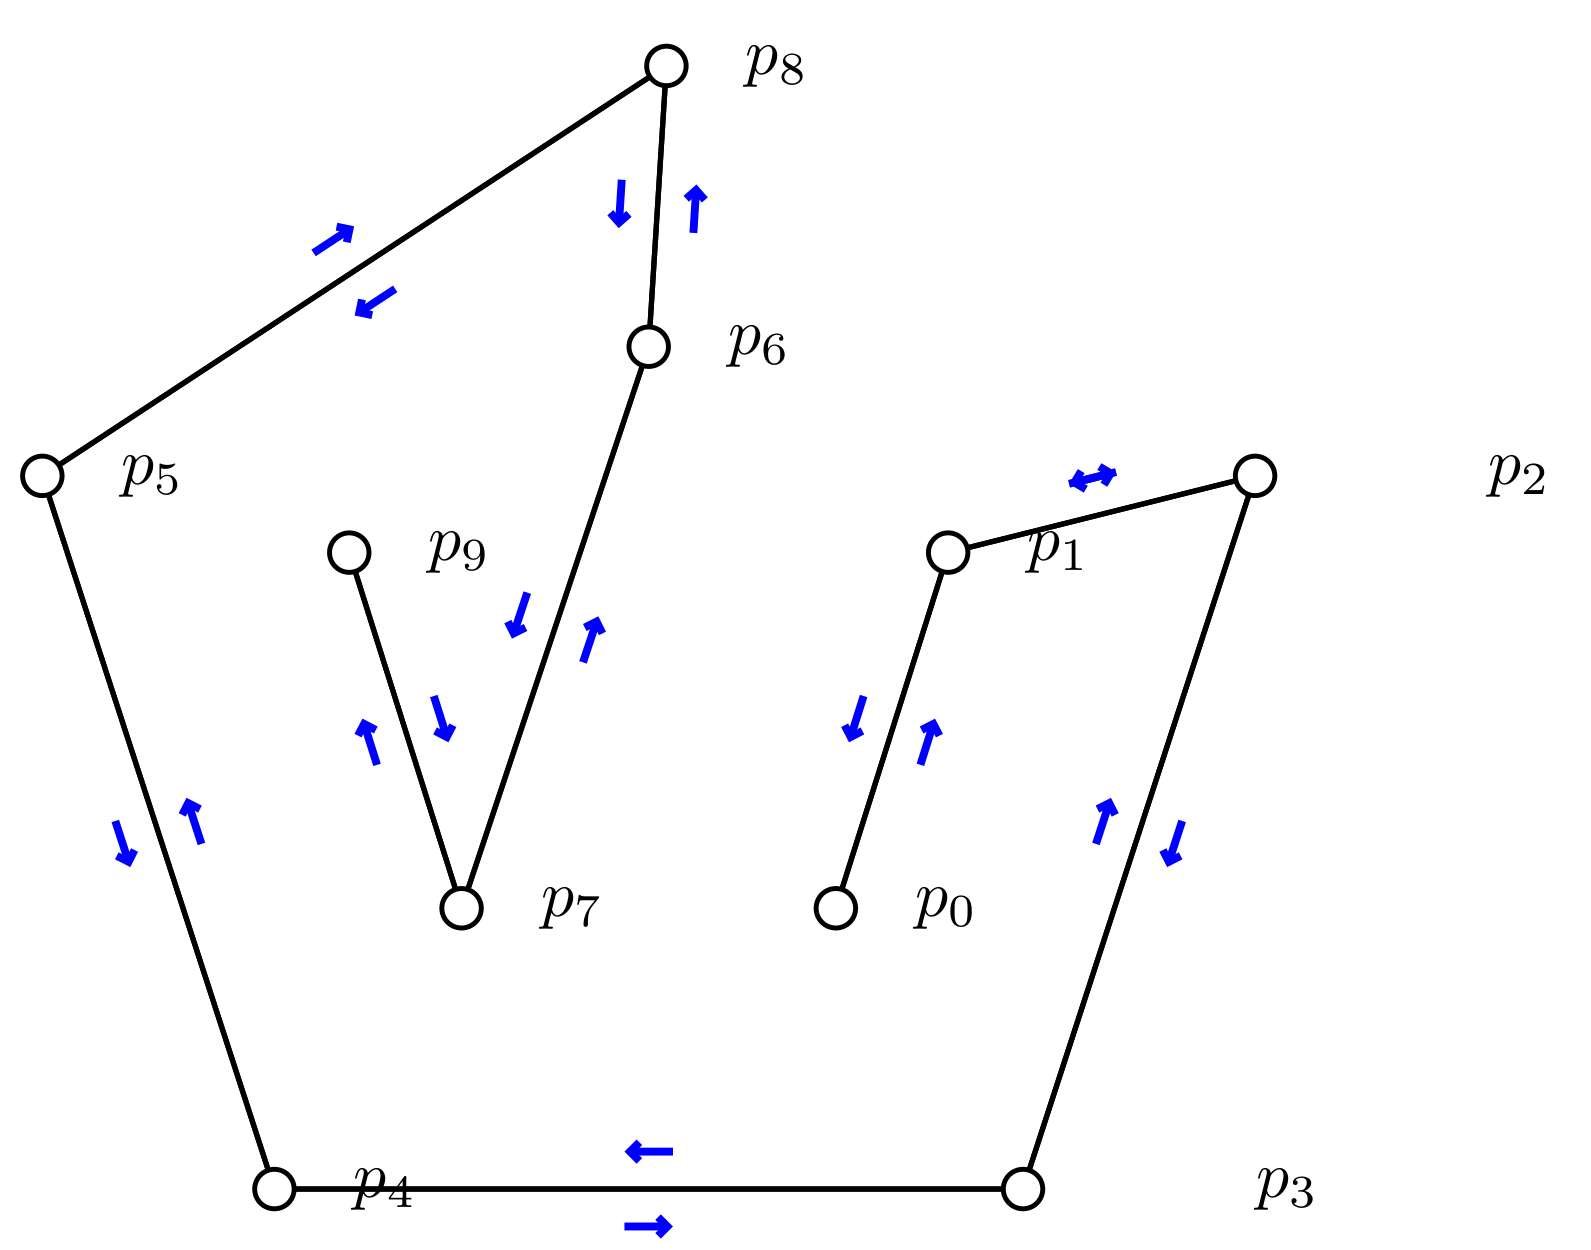
\includegraphics[width=7cm]{RD0.png}
                \caption{Gŕagica correspondiente a $R_0$.}
        \end{center}
\end{figure}

En la ronda ronda 1\footnote{$R_i$ representa a ``ronda $i$''.} tenemos
que:

\begin{multicols}{2}
\begin{itemize}
\item Estado de $p_0$:
      \begin{itemize}
      %%%%%%%%%%%%%%%% M
      \item \code{M = $\{\langle ID_1, \bot \rangle\}$}
      
      %%%%%%%%%%%%%%%% A
      \item \code{A = $\{ID_1\}$}
      
      %%%%%%%%%%%%%%%% C
      \item \code{C = $\bot$}
      \end{itemize}
      
\item Estado de $p_1$:
      \begin{itemize}
      %%%%%%%%%%%%%%%% M
      \item \code{M = $\{\langle ID_0, \bot \rangle,\;
                         \langle ID_2, \bot \rangle\}$}
      
      %%%%%%%%%%%%%%%% A
      \item \code{A = $\{ID_0,\; ID_2\}$}
      
      %%%%%%%%%%%%%%%% C
      \item \code{C = $\bot$}
      \end{itemize}

\item Estado de $p_2$:
      \begin{itemize}
      %%%%%%%%%%%%%%%% M
      \item \code{M = $\{\langle ID_1, \bot \rangle,\;
                         \langle ID_3, \bot \rangle\}$}
      
      %%%%%%%%%%%%%%%% A
      \item \code{A = $\{ID_1,\; ID_3\}$}
      
      %%%%%%%%%%%%%%%% C
      \item \code{C = $\bot$}
      \end{itemize}

\item Estado de $p_3$:
      \begin{itemize}
      %%%%%%%%%%%%%%%% M
      \item \code{M = $\{\langle ID_2, \bot \rangle,\;
                         \langle ID_4, \bot \rangle\}$}
      
      %%%%%%%%%%%%%%%% A
      \item \code{A = $\{ID_2,\; ID_4\}$}
      
      %%%%%%%%%%%%%%%% C
      \item \code{C = $\bot$}
      \end{itemize}

\item Estado de $p_4$:
      \begin{itemize}
      %%%%%%%%%%%%%%%% M
      \item \code{M = $\{\langle ID_3, \bot \rangle,\;
                         \langle ID_5, \bot \rangle\}$}
      
      %%%%%%%%%%%%%%%% A
      \item \code{A = $\{ID_3,\; ID_5\}$}
      
      %%%%%%%%%%%%%%%% C
      \item \code{C = $\bot$}
      \end{itemize}

\item Estado de $p_5$:
      \begin{itemize}
      %%%%%%%%%%%%%%%% M
      \item \code{M = $\{\langle ID_4, \bot \rangle,\;
                         \langle ID_8, \bot \rangle\}$}
      
      %%%%%%%%%%%%%%%% A
      \item \code{A = $\{ID_4,\; ID_8\}$}
      
      %%%%%%%%%%%%%%%% C
      \item \code{C = $\bot$}
      \end{itemize}

\item Estado de $p_6$:
      \begin{itemize}
      %%%%%%%%%%%%%%%% M
      \item \code{M = $\{\langle ID_7, \bot \rangle,\;
                         \langle ID_8, \bot \rangle\}$}
      
      %%%%%%%%%%%%%%%% A
      \item \code{A = $\{ID_7,\; ID_8\}$}
      
      %%%%%%%%%%%%%%%% C
      \item \code{C = $\bot$}
      \end{itemize}

\item Estado de $p_7$:
      \begin{itemize}
      %%%%%%%%%%%%%%%% M
      \item \code{M = $\{\langle ID_6, \bot \rangle,\;
                         \langle ID_9, \bot \rangle\}$}
      
      %%%%%%%%%%%%%%%% A
      \item \code{A = $\{ID_6, ID_9\}$}
      
      %%%%%%%%%%%%%%%% C
      \item \code{C = $\bot$}
      \end{itemize}

\item Estado de $p_8$:
      \begin{itemize}
      %%%%%%%%%%%%%%%% M
      \item \code{M = $\{\langle ID_5, \bot \rangle,\;
                         \langle ID_6, \bot \rangle\}$}
      
      %%%%%%%%%%%%%%%% A
      \item \code{A = $\{ID_5,\; ID_6\}$}
      
      %%%%%%%%%%%%%%%% C
      \item \code{C = $1$}
      \end{itemize}

\item Estado de $p_9$:
      \begin{itemize}
      %%%%%%%%%%%%%%%% M
      \item \code{M = $\{\langle ID_7, \bot \rangle\}$}
      
      %%%%%%%%%%%%%%%% A
      \item \code{A = $\{ID_7\}$}
      
      %%%%%%%%%%%%%%%% C
      \item \code{C = $1$}
      \end{itemize}

\end{itemize}
\end{multicols} 
\newpage

\begin{figure}[ht]
        \begin{center}
                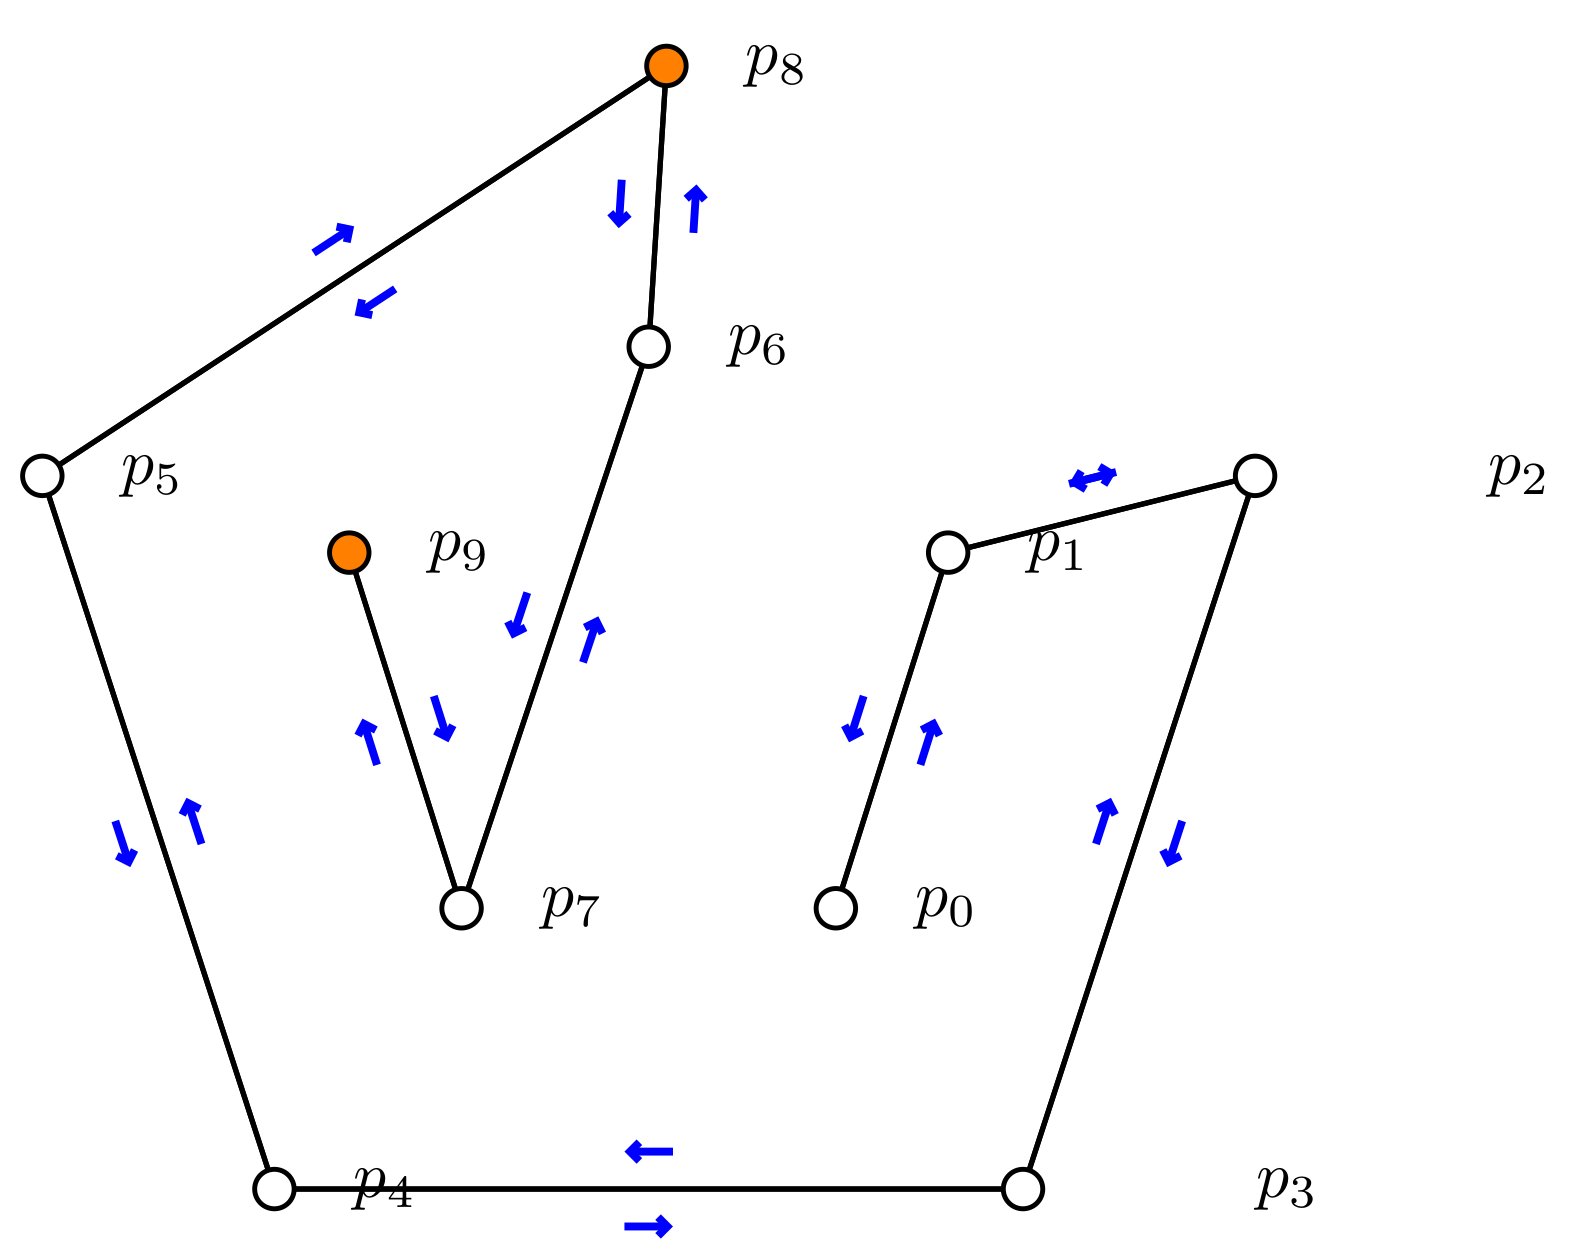
\includegraphics[width=7cm]{RD1.png}
                \caption{Gŕagica correspondiente a $R_1$.}
        \end{center}
\end{figure}

En la ronda ronda 2 tenemos que:

\begin{multicols}{2}
\begin{itemize}
\item Estado de $p_0$:
      \begin{itemize}
      %%%%%%%%%%%%%%%% M
      \item \code{M = $\{\langle ID_1, \bot \rangle\}$}
      
      %%%%%%%%%%%%%%%% A
      \item \code{A = $\{ID_1\}$}
      
      %%%%%%%%%%%%%%%% C
      \item \code{C = $\bot$}
      \end{itemize}
      
\item Estado de $p_1$:
      \begin{itemize}
      %%%%%%%%%%%%%%%% M
      \item \code{M = $\{\langle ID_0, \bot \rangle,\;
                         \langle ID_2, \bot \rangle\}$}
      
      %%%%%%%%%%%%%%%% A
      \item \code{A = $\{ID_0,\; ID_2\}$}
      
      %%%%%%%%%%%%%%%% C
      \item \code{C = $\bot$}
      \end{itemize}

\item Estado de $p_2$:
      \begin{itemize}
      %%%%%%%%%%%%%%%% M
      \item \code{M = $\{\langle ID_1, \bot \rangle,\;
                         \langle ID_3, \bot \rangle\}$}
      
      %%%%%%%%%%%%%%%% A
      \item \code{A = $\{ID_1,\; ID_3\}$}
      
      %%%%%%%%%%%%%%%% C
      \item \code{C = $\bot$}
      \end{itemize}

\item Estado de $p_3$:
      \begin{itemize}
      %%%%%%%%%%%%%%%% M
      \item \code{M = $\{\langle ID_2, \bot \rangle,\;
                         \langle ID_4, \bot \rangle\}$}
      
      %%%%%%%%%%%%%%%% A
      \item \code{A = $\{ID_2,\; ID_4\}$}
      
      %%%%%%%%%%%%%%%% C
      \item \code{C = $\bot$}
      \end{itemize}

\item Estado de $p_4$:
      \begin{itemize}
      %%%%%%%%%%%%%%%% M
      \item \code{M = $\{\langle ID_3, \bot \rangle,\;
                         \langle ID_5, \bot \rangle\}$}
      
      %%%%%%%%%%%%%%%% A
      \item \code{A = $\{ID_3,\; ID_5\}$}
      
      %%%%%%%%%%%%%%%% C
      \item \code{C = $\bot$}
      \end{itemize}

\item Estado de $p_5$:
      \begin{itemize}
      %%%%%%%%%%%%%%%% M
      \item \code{M = $\{\langle ID_4, \bot \rangle,\;
                         \langle ID_8, 1 \rangle\}$}
      
      %%%%%%%%%%%%%%%% A
      \item \code{A = $\{ID_4\}$}
      
      %%%%%%%%%%%%%%%% C
      \item \code{C = $2$}
      \end{itemize}

\item Estado de $p_6$:
      \begin{itemize}
      %%%%%%%%%%%%%%%% M
      \item \code{M = $\{\langle ID_7, \bot \rangle,\;
                         \langle ID_8, 1 \rangle\}$}
      
      %%%%%%%%%%%%%%%% A
      \item \code{A = $\{ID_7\}$}
      
      %%%%%%%%%%%%%%%% C
      \item \code{C = $\bot$}
      \end{itemize}

\item Estado de $p_7$:
      \begin{itemize}
      %%%%%%%%%%%%%%%% M
      \item \code{M = $\{\langle ID_6, \bot \rangle,\;
                         \langle ID_9, 1 \rangle\}$}
      
      %%%%%%%%%%%%%%%% A
      \item \code{A = $\{ID_6\}$}
      
      %%%%%%%%%%%%%%%% C
      \item \code{C = $2$}
      \end{itemize}

\item Estado de $p_8$:
      \begin{itemize}
      %%%%%%%%%%%%%%%% M
      \item \code{M = $\{\langle ID_5, \bot \rangle,\;
                         \langle ID_6, \bot \rangle\}$}
      
      %%%%%%%%%%%%%%%% A
      \item \code{A = $\{ID_5,\; ID_6\}$}
      
      %%%%%%%%%%%%%%%% C
      \item \code{C = $1$}
      \end{itemize}

\item Estado de $p_9$:
      \begin{itemize}
      %%%%%%%%%%%%%%%% M
      \item \code{M = $\{\langle ID_7, \bot \rangle\}$}
      
      %%%%%%%%%%%%%%%% A
      \item \code{A = $\{ID_7\}$}
      
      %%%%%%%%%%%%%%%% C
      \item \code{C = $1$}
      \end{itemize}

\end{itemize}
\end{multicols} 
\newpage

\begin{figure}[ht]
        \begin{center}
                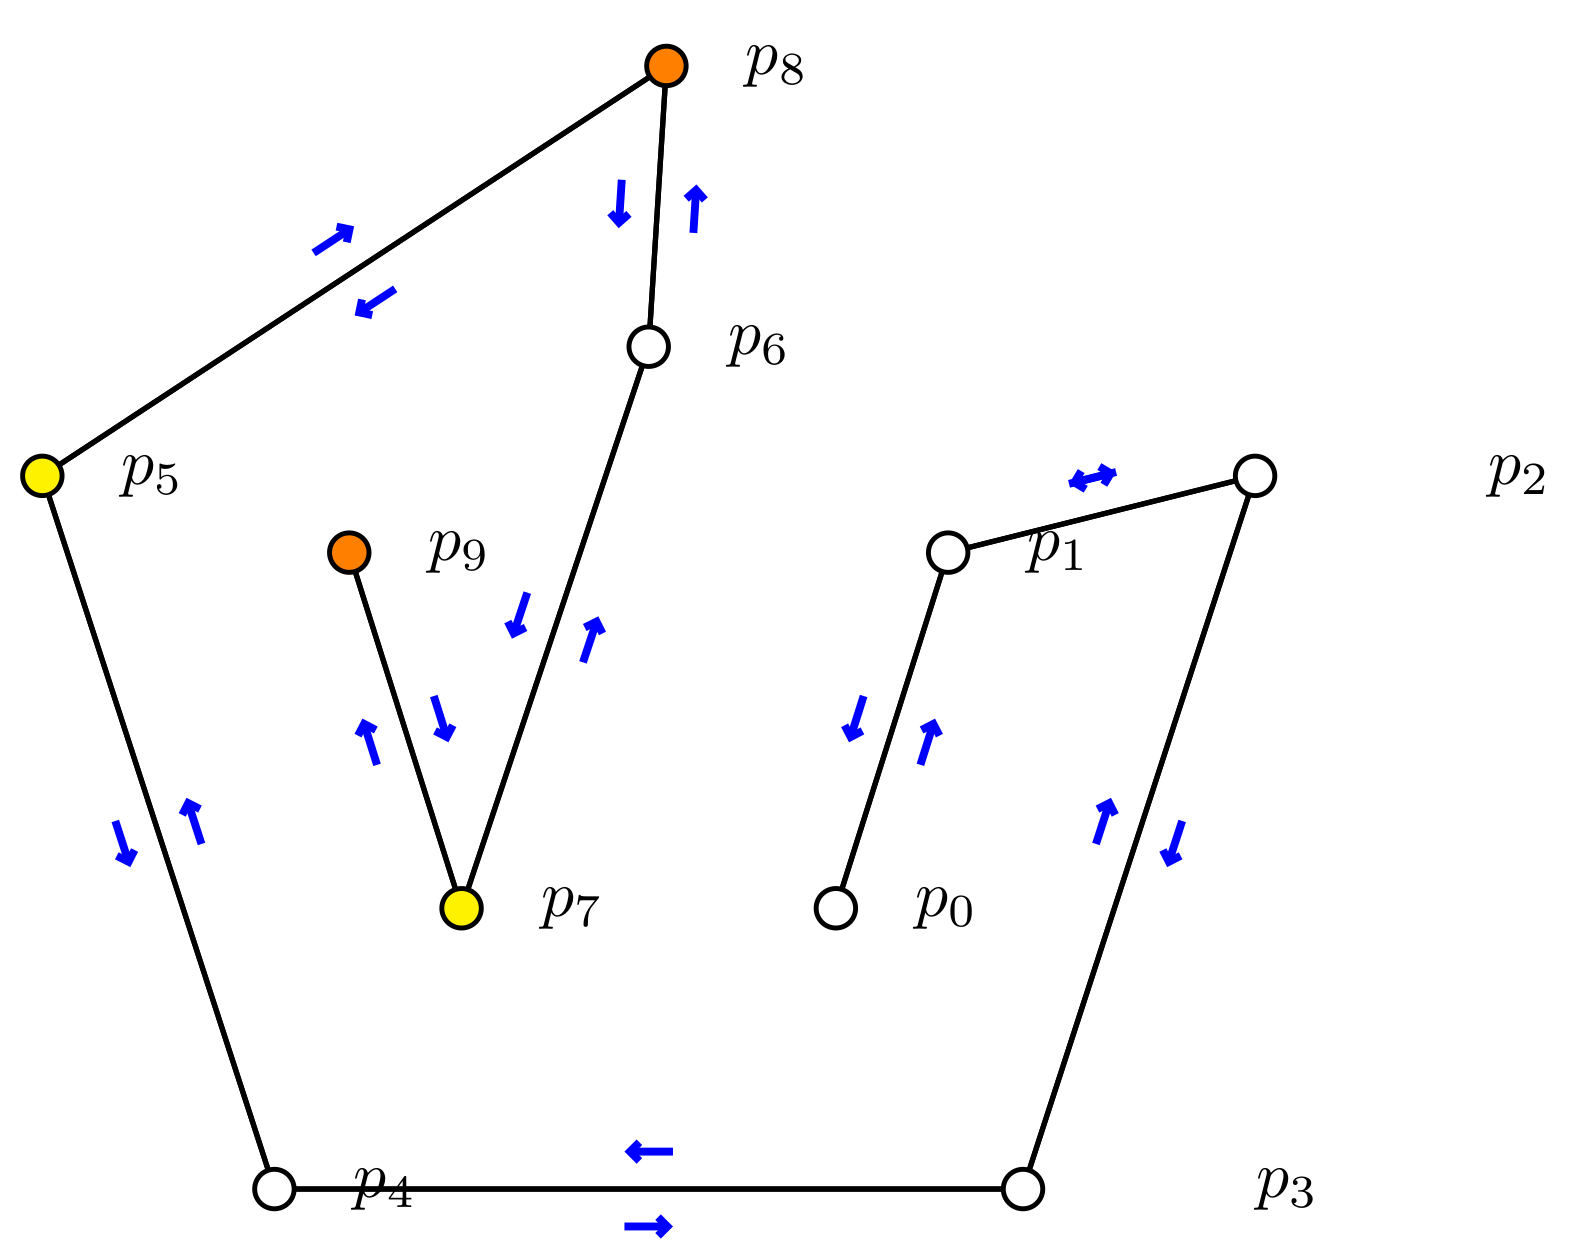
\includegraphics[width=7cm]{RD2.png}
                \caption{Gŕagica correspondiente a $R_2$.}
        \end{center}
\end{figure}

En la ronda 3 tenemos que:

\begin{multicols}{2}
\begin{itemize}
\item Estado de $p_0$:
      \begin{itemize}
      %%%%%%%%%%%%%%%% M
      \item \code{M = $\{\langle ID_1, \bot \rangle\}$}
      
      %%%%%%%%%%%%%%%% A
      \item \code{A = $\{ID_1\}$}
      
      %%%%%%%%%%%%%%%% C
      \item \code{C = $\bot$}
      \end{itemize}
      
\item Estado de $p_1$:
      \begin{itemize}
      %%%%%%%%%%%%%%%% M
      \item \code{M = $\{\langle ID_0, \bot \rangle,\;
                         \langle ID_2, \bot \rangle\}$}
      
      %%%%%%%%%%%%%%%% A
      \item \code{A = $\{ID_0,\; ID_2\}$}
      
      %%%%%%%%%%%%%%%% C
      \item \code{C = $\bot$}
      \end{itemize}

\item Estado de $p_2$:
      \begin{itemize}
      %%%%%%%%%%%%%%%% M
      \item \code{M = $\{\langle ID_1, \bot \rangle,\;
                         \langle ID_3, \bot \rangle\}$}
      
      %%%%%%%%%%%%%%%% A
      \item \code{A = $\{ID_1,\; ID_3\}$}
      
      %%%%%%%%%%%%%%%% C
      \item \code{C = $\bot$}
      \end{itemize}

\item Estado de $p_3$:
      \begin{itemize}
      %%%%%%%%%%%%%%%% M
      \item \code{M = $\{\langle ID_2, \bot \rangle,\;
                         \langle ID_4, \bot \rangle\}$}
      
      %%%%%%%%%%%%%%%% A
      \item \code{A = $\{ID_2,\; ID_4\}$}
      
      %%%%%%%%%%%%%%%% C
      \item \code{C = $\bot$}
      \end{itemize}

\item Estado de $p_4$:
      \begin{itemize}
      %%%%%%%%%%%%%%%% M
      \item \code{M = $\{\langle ID_3, \bot \rangle,\;
                         \langle ID_5, 2 \rangle\}$}
      
      %%%%%%%%%%%%%%%% A
      \item \code{A = $\{ID_3\}$}
      
      %%%%%%%%%%%%%%%% C
      \item \code{C = $1$}
      \end{itemize}

\item Estado de $p_5$:
      \begin{itemize}
      %%%%%%%%%%%%%%%% M
      \item \code{M = $\{\langle ID_4, \bot \rangle,\;
                         \langle ID_8, 1 \rangle\}$}
      
      %%%%%%%%%%%%%%%% A
      \item \code{A = $\{ID_4\}$}
      
      %%%%%%%%%%%%%%%% C
      \item \code{C = $1$}
      \end{itemize}

\item Estado de $p_6$:
      \begin{itemize}
      %%%%%%%%%%%%%%%% M
      \item \code{M = $\{\langle ID_7, 2 \rangle,\;
                         \langle ID_8, 1 \rangle\}$}
      
      %%%%%%%%%%%%%%%% A
      \item \code{A = $\emptyset$}
      
      %%%%%%%%%%%%%%%% C
      \item \code{C = $3$}
      \end{itemize}

\item Estado de $p_7$:
      \begin{itemize}
      %%%%%%%%%%%%%%%% M
      \item \code{M = $\{\langle ID_6, \bot \rangle,\;
                         \langle ID_9, 1 \rangle\}$}
      
      %%%%%%%%%%%%%%%% A
      \item \code{A = $\{ID_6\}$}
      
      %%%%%%%%%%%%%%%% C
      \item \code{C = $2$}
      \end{itemize}

\item Estado de $p_8$:
      \begin{itemize}
      %%%%%%%%%%%%%%%% M
      \item \code{M = $\{\langle ID_5, 2 \rangle,\;
                         \langle ID_6, \bot \rangle\}$}
      
      %%%%%%%%%%%%%%%% A
      \item \code{A = $\{ID_6\}$}
      
      %%%%%%%%%%%%%%%% C
      \item \code{C = $1$}
      \end{itemize}

\item Estado de $p_9$:
      \begin{itemize}
      %%%%%%%%%%%%%%%% M
      \item \code{M = $\{\langle ID_7, 2 \rangle\}$}
      
      %%%%%%%%%%%%%%%% A
      \item \code{A = $\emptyset$}
      
      %%%%%%%%%%%%%%%% C
      \item \code{C = $1$}
      \end{itemize}

\end{itemize}
\end{multicols} 
\newpage

\begin{figure}[ht]
        \begin{center}
                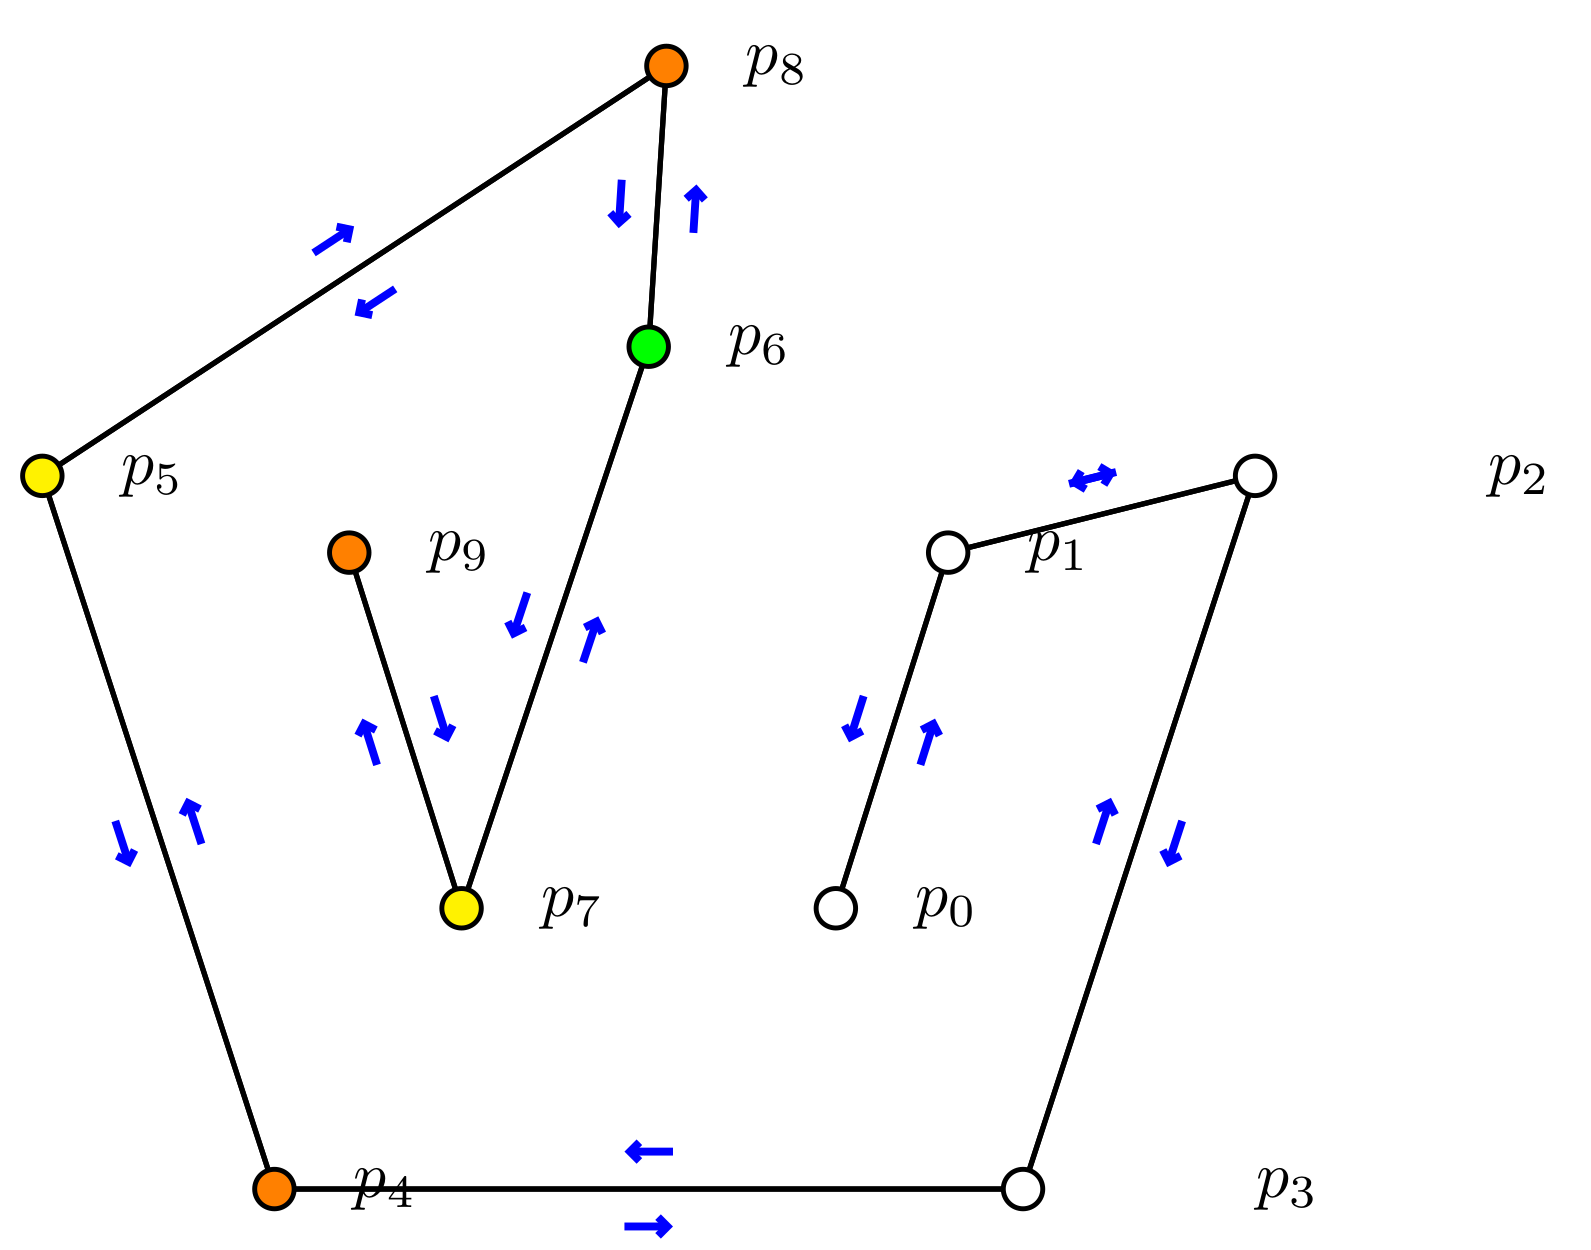
\includegraphics[width=7cm]{RD3.png}
                \caption{Gŕagica correspondiente a $R_3$.}
        \end{center}
\end{figure}

En la ronda 4 tenemos que:

\begin{multicols}{2}
\begin{itemize}
\item Estado de $p_0$:
      \begin{itemize}
      %%%%%%%%%%%%%%%% M
      \item \code{M = $\{\langle ID_1, \bot \rangle\}$}
      
      %%%%%%%%%%%%%%%% A
      \item \code{A = $\{ID_1\}$}
      
      %%%%%%%%%%%%%%%% C
      \item \code{C = $\bot$}
      \end{itemize}
      
\item Estado de $p_1$:
      \begin{itemize}
      %%%%%%%%%%%%%%%% M
      \item \code{M = $\{\langle ID_0, \bot \rangle,\;
                         \langle ID_2, \bot \rangle\}$}
      
      %%%%%%%%%%%%%%%% A
      \item \code{A = $\{ID_0,\; ID_2\}$}
      
      %%%%%%%%%%%%%%%% C
      \item \code{C = $\bot$}
      \end{itemize}

\item Estado de $p_2$:
      \begin{itemize}
      %%%%%%%%%%%%%%%% M
      \item \code{M = $\{\langle ID_1, \bot \rangle,\;
                         \langle ID_3, \bot \rangle\}$}
      
      %%%%%%%%%%%%%%%% A
      \item \code{A = $\{ID_1,\; ID_3\}$}
      
      %%%%%%%%%%%%%%%% C
      \item \code{C = $\bot$}
      \end{itemize}

\item Estado de $p_3$:
      \begin{itemize}
      %%%%%%%%%%%%%%%% M
      \item \code{M = $\{\langle ID_2, \bot \rangle,\;
                         \langle ID_4, 1 \rangle\}$}
      
      %%%%%%%%%%%%%%%% A
      \item \code{A = $\{ID_2\}$}
      
      %%%%%%%%%%%%%%%% C
      \item \code{C = $2$}
      \end{itemize}

\item Estado de $p_4$:
      \begin{itemize}
      %%%%%%%%%%%%%%%% M
      \item \code{M = $\{\langle ID_3, \bot \rangle,\;
                         \langle ID_5, 2 \rangle\}$}
      
      %%%%%%%%%%%%%%%% A
      \item \code{A = $\{ID_3\}$}
      
      %%%%%%%%%%%%%%%% C
      \item \code{C = $1$}
      \end{itemize}

\item Estado de $p_5$:
      \begin{itemize}
      %%%%%%%%%%%%%%%% M
      \item \code{M = $\{\langle ID_4, 1 \rangle,\;
                         \langle ID_8, 1 \rangle\}$}
      
      %%%%%%%%%%%%%%%% A
      \item \code{A = $\emptyset$}
      
      %%%%%%%%%%%%%%%% C
      \item \code{C = $1$}
      \end{itemize}

\item Estado de $p_6$:
      \begin{itemize}
      %%%%%%%%%%%%%%%% M
      \item \code{M = $\{\langle ID_7, 2 \rangle,\;
                         \langle ID_8, 1 \rangle\}$}
      
      %%%%%%%%%%%%%%%% A
      \item \code{A = $\emptyset$}
      
      %%%%%%%%%%%%%%%% C
      \item \code{C = $3$}
      \end{itemize}

\item Estado de $p_7$:
      \begin{itemize}
      %%%%%%%%%%%%%%%% M
      \item \code{M = $\{\langle ID_6, 3 \rangle,\;
                         \langle ID_9, 1 \rangle\}$}
      
      %%%%%%%%%%%%%%%% A
      \item \code{A = $\emptyset$}
      
      %%%%%%%%%%%%%%%% C
      \item \code{C = $2$}
      \end{itemize}

\item Estado de $p_8$:
      \begin{itemize}
      %%%%%%%%%%%%%%%% M
      \item \code{M = $\{\langle ID_5, 2 \rangle,\;
                         \langle ID_6, 3 \rangle\}$}
      
      %%%%%%%%%%%%%%%% A
      \item \code{A = $\emptyset$}
      
      %%%%%%%%%%%%%%%% C
      \item \code{C = $1$}
      \end{itemize}

\item Estado de $p_9$:
      \begin{itemize}
      %%%%%%%%%%%%%%%% M
      \item \code{M = $\{\langle ID_7, 2 \rangle\}$}
      
      %%%%%%%%%%%%%%%% A
      \item \code{A = $\emptyset$}
      
      %%%%%%%%%%%%%%%% C
      \item \code{C = $1$}
      \end{itemize}

\end{itemize}
\end{multicols} 
\newpage

\begin{figure}[ht]
        \begin{center}
                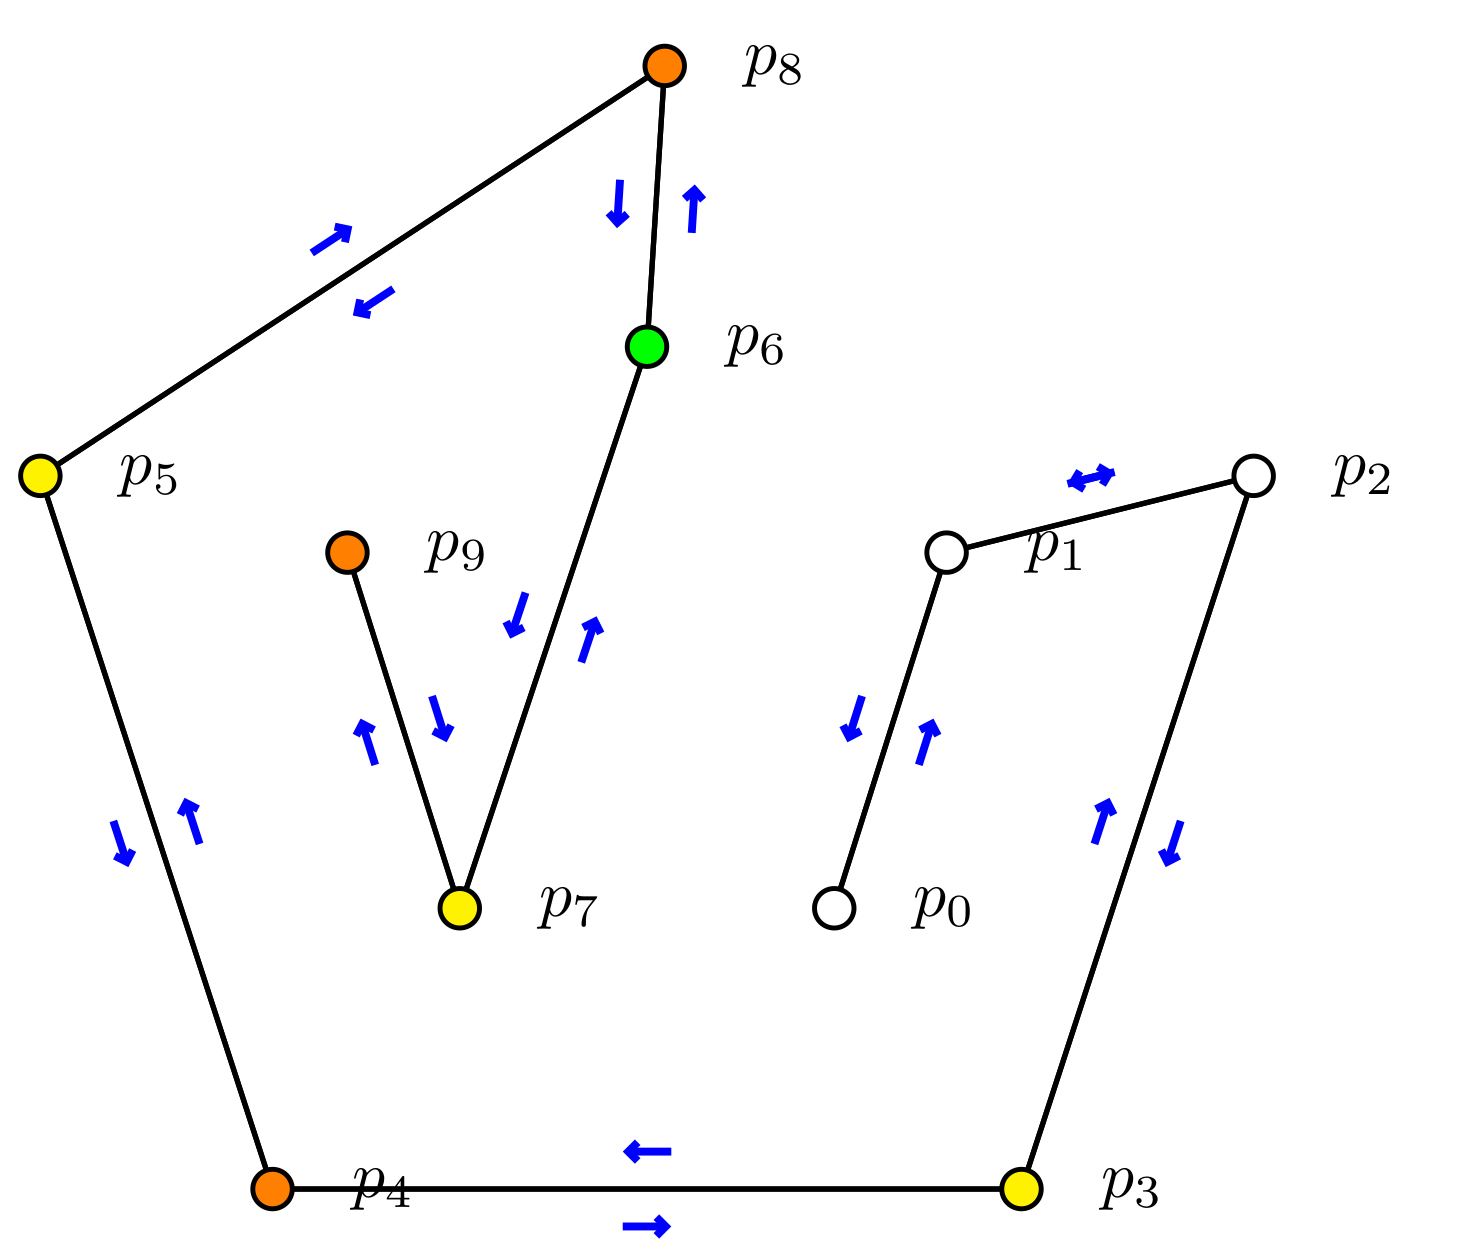
\includegraphics[width=7cm]{RD4.png}
                \caption{Gŕagica correspondiente a $R_4$.}
        \end{center}
\end{figure}

En la ronda 5 tenemos que:

\begin{multicols}{2}
\begin{itemize}
\item Estado de $p_0$:
      \begin{itemize}
      %%%%%%%%%%%%%%%% M
      \item \code{M = $\{\langle ID_1, \bot \rangle\}$}
      
      %%%%%%%%%%%%%%%% A
      \item \code{A = $\{ID_1\}$}
      
      %%%%%%%%%%%%%%%% C
      \item \code{C = $\bot$}
      \end{itemize}
      
\item Estado de $p_1$:
      \begin{itemize}
      %%%%%%%%%%%%%%%% M
      \item \code{M = $\{\langle ID_0, \bot \rangle,\;
                         \langle ID_2, \bot \rangle\}$}
      
      %%%%%%%%%%%%%%%% A
      \item \code{A = $\{ID_0,\; ID_2\}$}
      
      %%%%%%%%%%%%%%%% C
      \item \code{C = $\bot$}
      \end{itemize}

\item Estado de $p_2$:
      \begin{itemize}
      %%%%%%%%%%%%%%%% M
      \item \code{M = $\{\langle ID_1, \bot \rangle,\;
                         \langle ID_3, 2 \rangle\}$}
      
      %%%%%%%%%%%%%%%% A
      \item \code{A = $\{ID_1\}$}
      
      %%%%%%%%%%%%%%%% C
      \item \code{C = $1$}
      \end{itemize}

\item Estado de $p_3$:
      \begin{itemize}
      %%%%%%%%%%%%%%%% M
      \item \code{M = $\{\langle ID_2, \bot \rangle,\;
                         \langle ID_4, 1 \rangle\}$}
      
      %%%%%%%%%%%%%%%% A
      \item \code{A = $\{ID_2\}$}
      
      %%%%%%%%%%%%%%%% C
      \item \code{C = $2$}
      \end{itemize}

\item Estado de $p_4$:
      \begin{itemize}
      %%%%%%%%%%%%%%%% M
      \item \code{M = $\{\langle ID_3, 2 \rangle,\;
                         \langle ID_5, 2 \rangle\}$}
      
      %%%%%%%%%%%%%%%% A
      \item \code{A = $\emptyset$}
      
      %%%%%%%%%%%%%%%% C
      \item \code{C = $1$}
      \end{itemize}

\item Estado de $p_5$:
      \begin{itemize}
      %%%%%%%%%%%%%%%% M
      \item \code{M = $\{\langle ID_4, 1 \rangle,\;
                         \langle ID_8, 1 \rangle\}$}
      
      %%%%%%%%%%%%%%%% A
      \item \code{A = $\emptyset$}
      
      %%%%%%%%%%%%%%%% C
      \item \code{C = $1$}
      \end{itemize}

\item Estado de $p_6$:
      \begin{itemize}
      %%%%%%%%%%%%%%%% M
      \item \code{M = $\{\langle ID_7, 2 \rangle,\;
                         \langle ID_8, 1 \rangle\}$}
      
      %%%%%%%%%%%%%%%% A
      \item \code{A = $\emptyset$}
      
      %%%%%%%%%%%%%%%% C
      \item \code{C = $3$}
      \end{itemize}

\item Estado de $p_7$:
      \begin{itemize}
      %%%%%%%%%%%%%%%% M
      \item \code{M = $\{\langle ID_6, 3 \rangle,\;
                         \langle ID_9, 1 \rangle\}$}
      
      %%%%%%%%%%%%%%%% A
      \item \code{A = $\emptyset$}
      
      %%%%%%%%%%%%%%%% C
      \item \code{C = $2$}
      \end{itemize}

\item Estado de $p_8$:
      \begin{itemize}
      %%%%%%%%%%%%%%%% M
      \item \code{M = $\{\langle ID_5, 2 \rangle,\;
                         \langle ID_6, 3 \rangle\}$}
      
      %%%%%%%%%%%%%%%% A
      \item \code{A = $\emptyset$}
      
      %%%%%%%%%%%%%%%% C
      \item \code{C = $1$}
      \end{itemize}

\item Estado de $p_9$:
      \begin{itemize}
      %%%%%%%%%%%%%%%% M
      \item \code{M = $\{\langle ID_7, 2 \rangle\}$}
      
      %%%%%%%%%%%%%%%% A
      \item \code{A = $\emptyset$}
      
      %%%%%%%%%%%%%%%% C
      \item \code{C = $1$}
      \end{itemize}

\end{itemize}
\end{multicols} 
\newpage

\begin{figure}[ht]
        \begin{center}
                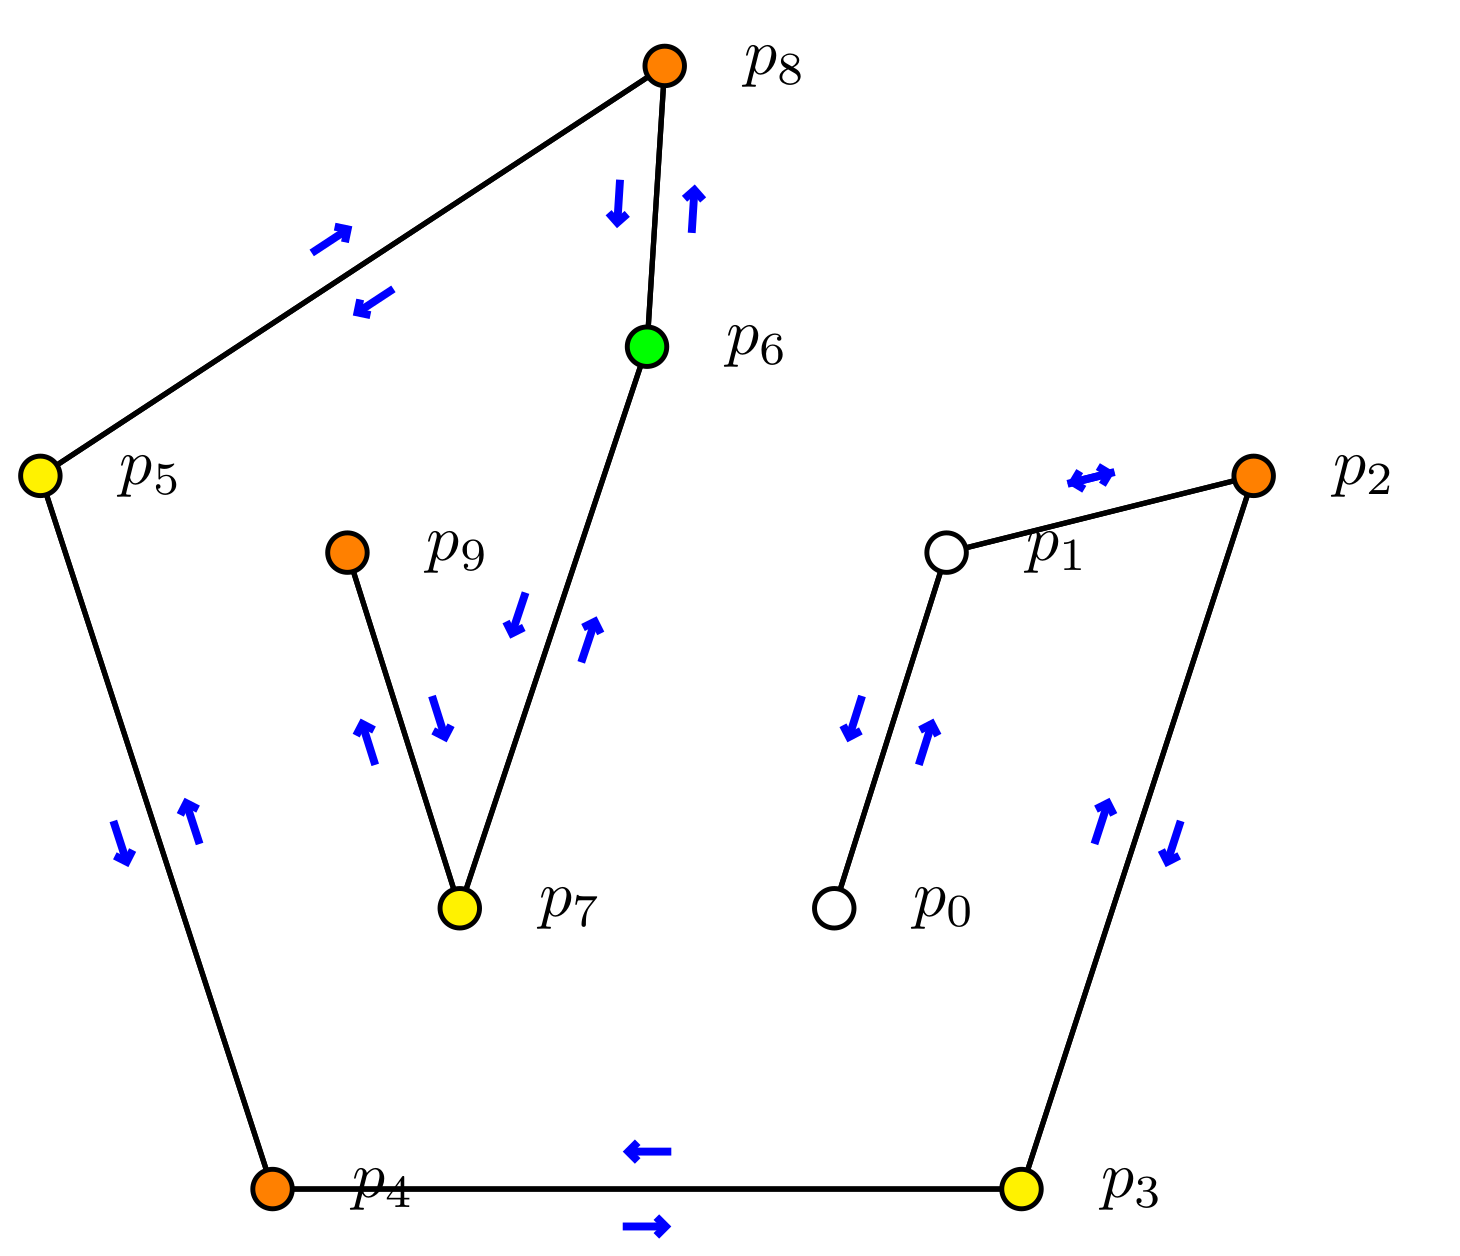
\includegraphics[width=7cm]{RD5.png}
                \caption{Gŕagica correspondiente a $R_5$.}
        \end{center}
\end{figure}

En la ronda 6 tenemos que:

\begin{multicols}{2}
\begin{itemize}
\item Estado de $p_0$:
      \begin{itemize}
      %%%%%%%%%%%%%%%% M
      \item \code{M = $\{\langle ID_1, \bot \rangle\}$}
      
      %%%%%%%%%%%%%%%% A
      \item \code{A = $\{ID_1\}$}
      
      %%%%%%%%%%%%%%%% C
      \item \code{C = $\bot$}
      \end{itemize}
      
\item Estado de $p_1$:
      \begin{itemize}
      %%%%%%%%%%%%%%%% M
      \item \code{M = $\{\langle ID_0, \bot \rangle,\;
                         \langle ID_2, 1 \rangle\}$}
      
      %%%%%%%%%%%%%%%% A
      \item \code{A = $\{ID_0\}$}
      
      %%%%%%%%%%%%%%%% C
      \item \code{C = $2$}
      \end{itemize}

\item Estado de $p_2$:
      \begin{itemize}
      %%%%%%%%%%%%%%%% M
      \item \code{M = $\{\langle ID_1, \bot \rangle,\;
                         \langle ID_3, 2 \rangle\}$}
      
      %%%%%%%%%%%%%%%% A
      \item \code{A = $\{ID_1\}$}
      
      %%%%%%%%%%%%%%%% C
      \item \code{C = $1$}
      \end{itemize}

\item Estado de $p_3$:
      \begin{itemize}
      %%%%%%%%%%%%%%%% M
      \item \code{M = $\{\langle ID_2, 1 \rangle,\;
                         \langle ID_4, 1 \rangle\}$}
      
      %%%%%%%%%%%%%%%% A
      \item \code{A = $\emptyset$}
      
      %%%%%%%%%%%%%%%% C
      \item \code{C = $2$}
      \end{itemize}

\item Estado de $p_4$:
      \begin{itemize}
      %%%%%%%%%%%%%%%% M
      \item \code{M = $\{\langle ID_3, 2 \rangle,\;
                         \langle ID_5, 2 \rangle\}$}
      
      %%%%%%%%%%%%%%%% A
      \item \code{A = $\emptyset$}
      
      %%%%%%%%%%%%%%%% C
      \item \code{C = $1$}
      \end{itemize}

\item Estado de $p_5$:
      \begin{itemize}
      %%%%%%%%%%%%%%%% M
      \item \code{M = $\{\langle ID_4, 1 \rangle,\;
                         \langle ID_8, 1 \rangle\}$}
      
      %%%%%%%%%%%%%%%% A
      \item \code{A = $\emptyset$}
      
      %%%%%%%%%%%%%%%% C
      \item \code{C = $1$}
      \end{itemize}

\item Estado de $p_6$:
      \begin{itemize}
      %%%%%%%%%%%%%%%% M
      \item \code{M = $\{\langle ID_7, 2 \rangle,\;
                         \langle ID_8, 1 \rangle\}$}
      
      %%%%%%%%%%%%%%%% A
      \item \code{A = $\emptyset$}
      
      %%%%%%%%%%%%%%%% C
      \item \code{C = $3$}
      \end{itemize}

\item Estado de $p_7$:
      \begin{itemize}
      %%%%%%%%%%%%%%%% M
      \item \code{M = $\{\langle ID_6, 3 \rangle,\;
                         \langle ID_9, 1 \rangle\}$}
      
      %%%%%%%%%%%%%%%% A
      \item \code{A = $\emptyset$}
      
      %%%%%%%%%%%%%%%% C
      \item \code{C = $2$}
      \end{itemize}

\item Estado de $p_8$:
      \begin{itemize}
      %%%%%%%%%%%%%%%% M
      \item \code{M = $\{\langle ID_5, 2 \rangle,\;
                         \langle ID_6, 3 \rangle\}$}
      
      %%%%%%%%%%%%%%%% A
      \item \code{A = $\emptyset$}
      
      %%%%%%%%%%%%%%%% C
      \item \code{C = $1$}
      \end{itemize}

\item Estado de $p_9$:
      \begin{itemize}
      %%%%%%%%%%%%%%%% M
      \item \code{M = $\{\langle ID_7, 2 \rangle\}$}
      
      %%%%%%%%%%%%%%%% A
      \item \code{A = $\emptyset$}
      
      %%%%%%%%%%%%%%%% C
      \item \code{C = $1$}
      \end{itemize}

\end{itemize}
\end{multicols} 
\newpage

\begin{figure}[ht]
        \begin{center}
                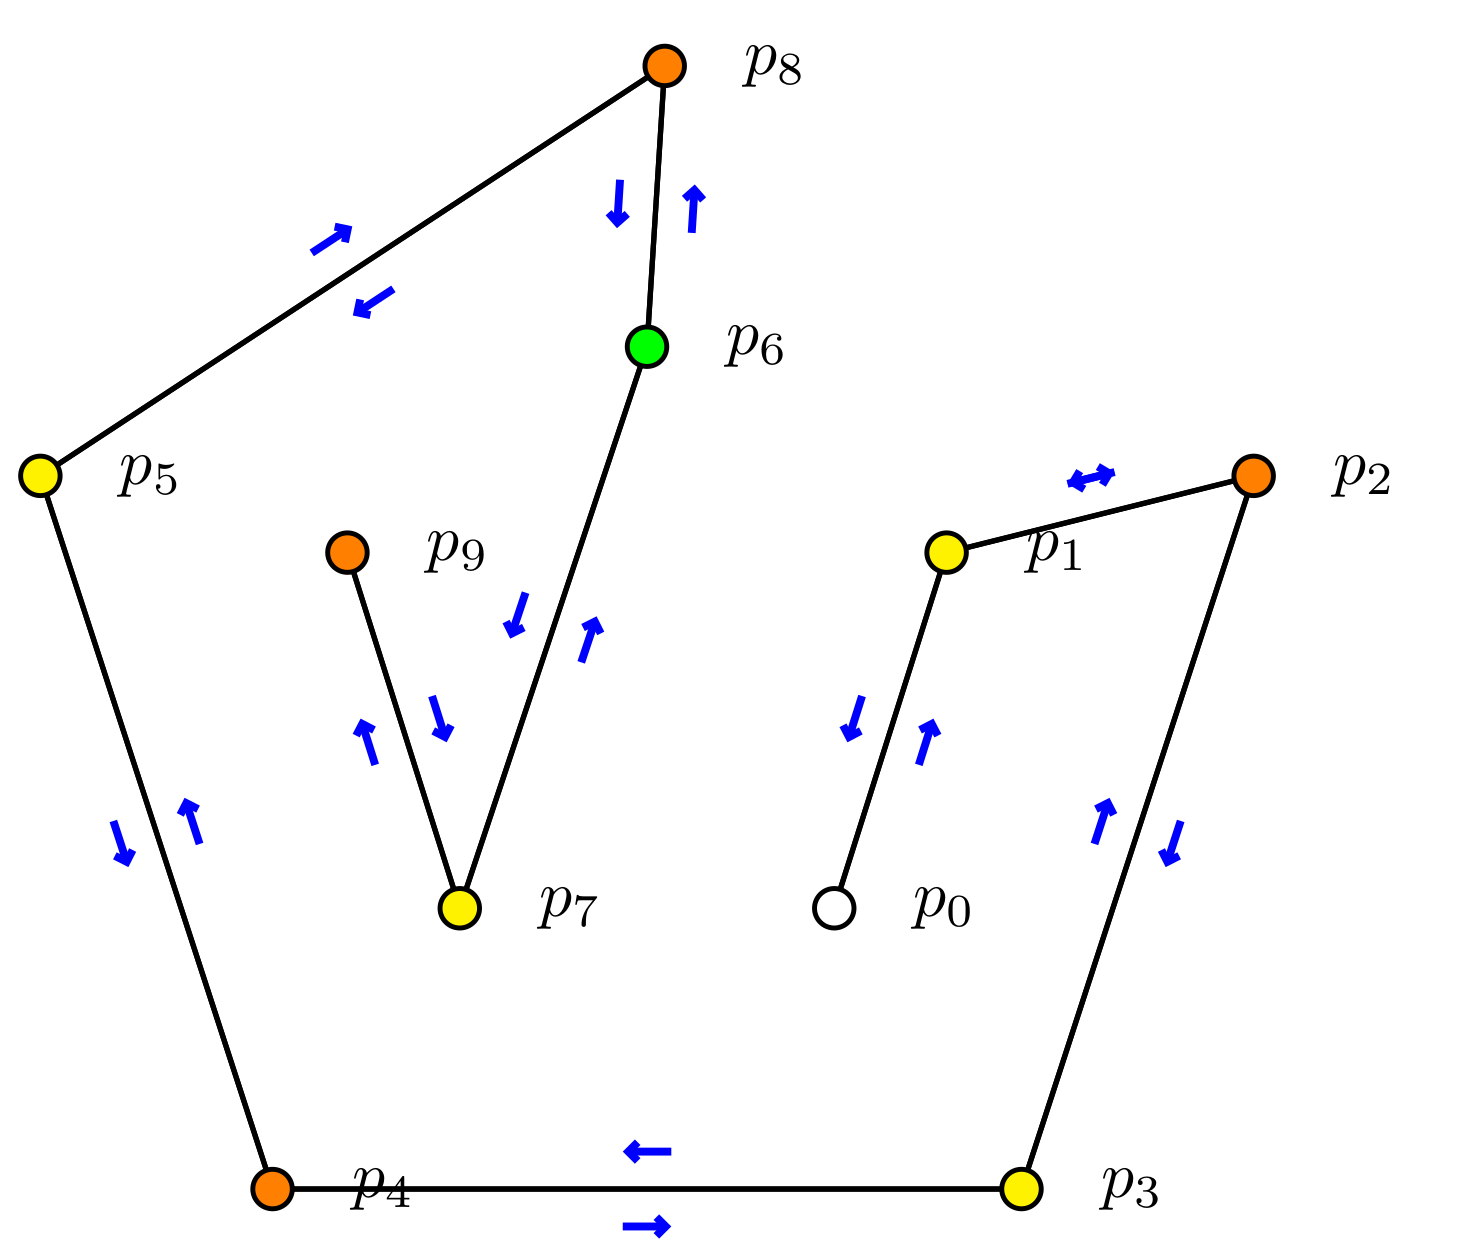
\includegraphics[width=7cm]{RD6.png}
                \caption{Gŕagica correspondiente a $R_6$.}
        \end{center}
\end{figure}

En la ronda 7 tenemos que:

\begin{multicols}{2}
\begin{itemize}
\item Estado de $p_0$:
      \begin{itemize}
      %%%%%%%%%%%%%%%% M
      \item \code{M = $\{\langle ID_1, 2 \rangle\}$}
      
      %%%%%%%%%%%%%%%% A
      \item \code{A = $\emptyset$}
      
      %%%%%%%%%%%%%%%% C
      \item \code{C = $1$}
      \end{itemize}
      
\item Estado de $p_1$:
      \begin{itemize}
      %%%%%%%%%%%%%%%% M
      \item \code{M = $\{\langle ID_0, \bot \rangle,\;
                         \langle ID_2, 1 \rangle\}$}
      
      %%%%%%%%%%%%%%%% A
      \item \code{A = $\{ID_0\}$}
      
      %%%%%%%%%%%%%%%% C
      \item \code{C = $2$}
      \end{itemize}

\item Estado de $p_2$:
      \begin{itemize}
      %%%%%%%%%%%%%%%% M
      \item \code{M = $\{\langle ID_1, 2 \rangle,\;
                         \langle ID_3, 2 \rangle\}$}
      
      %%%%%%%%%%%%%%%% A
      \item \code{A = $\emptyset$}
      
      %%%%%%%%%%%%%%%% C
      \item \code{C = $1$}
      \end{itemize}

\item Estado de $p_3$:
      \begin{itemize}
      %%%%%%%%%%%%%%%% M
      \item \code{M = $\{\langle ID_2, 1 \rangle,\;
                         \langle ID_4, 1 \rangle\}$}
      
      %%%%%%%%%%%%%%%% A
      \item \code{A = $\emptyset$}
      
      %%%%%%%%%%%%%%%% C
      \item \code{C = $2$}
      \end{itemize}

\item Estado de $p_4$:
      \begin{itemize}
      %%%%%%%%%%%%%%%% M
      \item \code{M = $\{\langle ID_3, 2 \rangle,\;
                         \langle ID_5, 2 \rangle\}$}
      
      %%%%%%%%%%%%%%%% A
      \item \code{A = $\emptyset$}
      
      %%%%%%%%%%%%%%%% C
      \item \code{C = $1$}
      \end{itemize}

\item Estado de $p_5$:
      \begin{itemize}
      %%%%%%%%%%%%%%%% M
      \item \code{M = $\{\langle ID_4, 1 \rangle,\;
                         \langle ID_8, 1 \rangle\}$}
      
      %%%%%%%%%%%%%%%% A
      \item \code{A = $\emptyset$}
      
      %%%%%%%%%%%%%%%% C
      \item \code{C = $1$}
      \end{itemize}

\item Estado de $p_6$:
      \begin{itemize}
      %%%%%%%%%%%%%%%% M
      \item \code{M = $\{\langle ID_7, 2 \rangle,\;
                         \langle ID_8, 1 \rangle\}$}
      
      %%%%%%%%%%%%%%%% A
      \item \code{A = $\emptyset$}
      
      %%%%%%%%%%%%%%%% C
      \item \code{C = $3$}
      \end{itemize}

\item Estado de $p_7$:
      \begin{itemize}
      %%%%%%%%%%%%%%%% M
      \item \code{M = $\{\langle ID_6, 3 \rangle,\;
                         \langle ID_9, 1 \rangle\}$}
      
      %%%%%%%%%%%%%%%% A
      \item \code{A = $\emptyset$}
      
      %%%%%%%%%%%%%%%% C
      \item \code{C = $2$}
      \end{itemize}

\item Estado de $p_8$:
      \begin{itemize}
      %%%%%%%%%%%%%%%% M
      \item \code{M = $\{\langle ID_5, 2 \rangle,\;
                         \langle ID_6, 3 \rangle\}$}
      
      %%%%%%%%%%%%%%%% A
      \item \code{A = $\emptyset$}
      
      %%%%%%%%%%%%%%%% C
      \item \code{C = $1$}
      \end{itemize}

\item Estado de $p_9$:
      \begin{itemize}
      %%%%%%%%%%%%%%%% M
      \item \code{M = $\{\langle ID_7, 2 \rangle\}$}
      
      %%%%%%%%%%%%%%%% A
      \item \code{A = $\emptyset$}
      
      %%%%%%%%%%%%%%%% C
      \item \code{C = $1$}
      \end{itemize}

\end{itemize}
\end{multicols} 
\newpage

\begin{figure}[ht]
        \begin{center}
                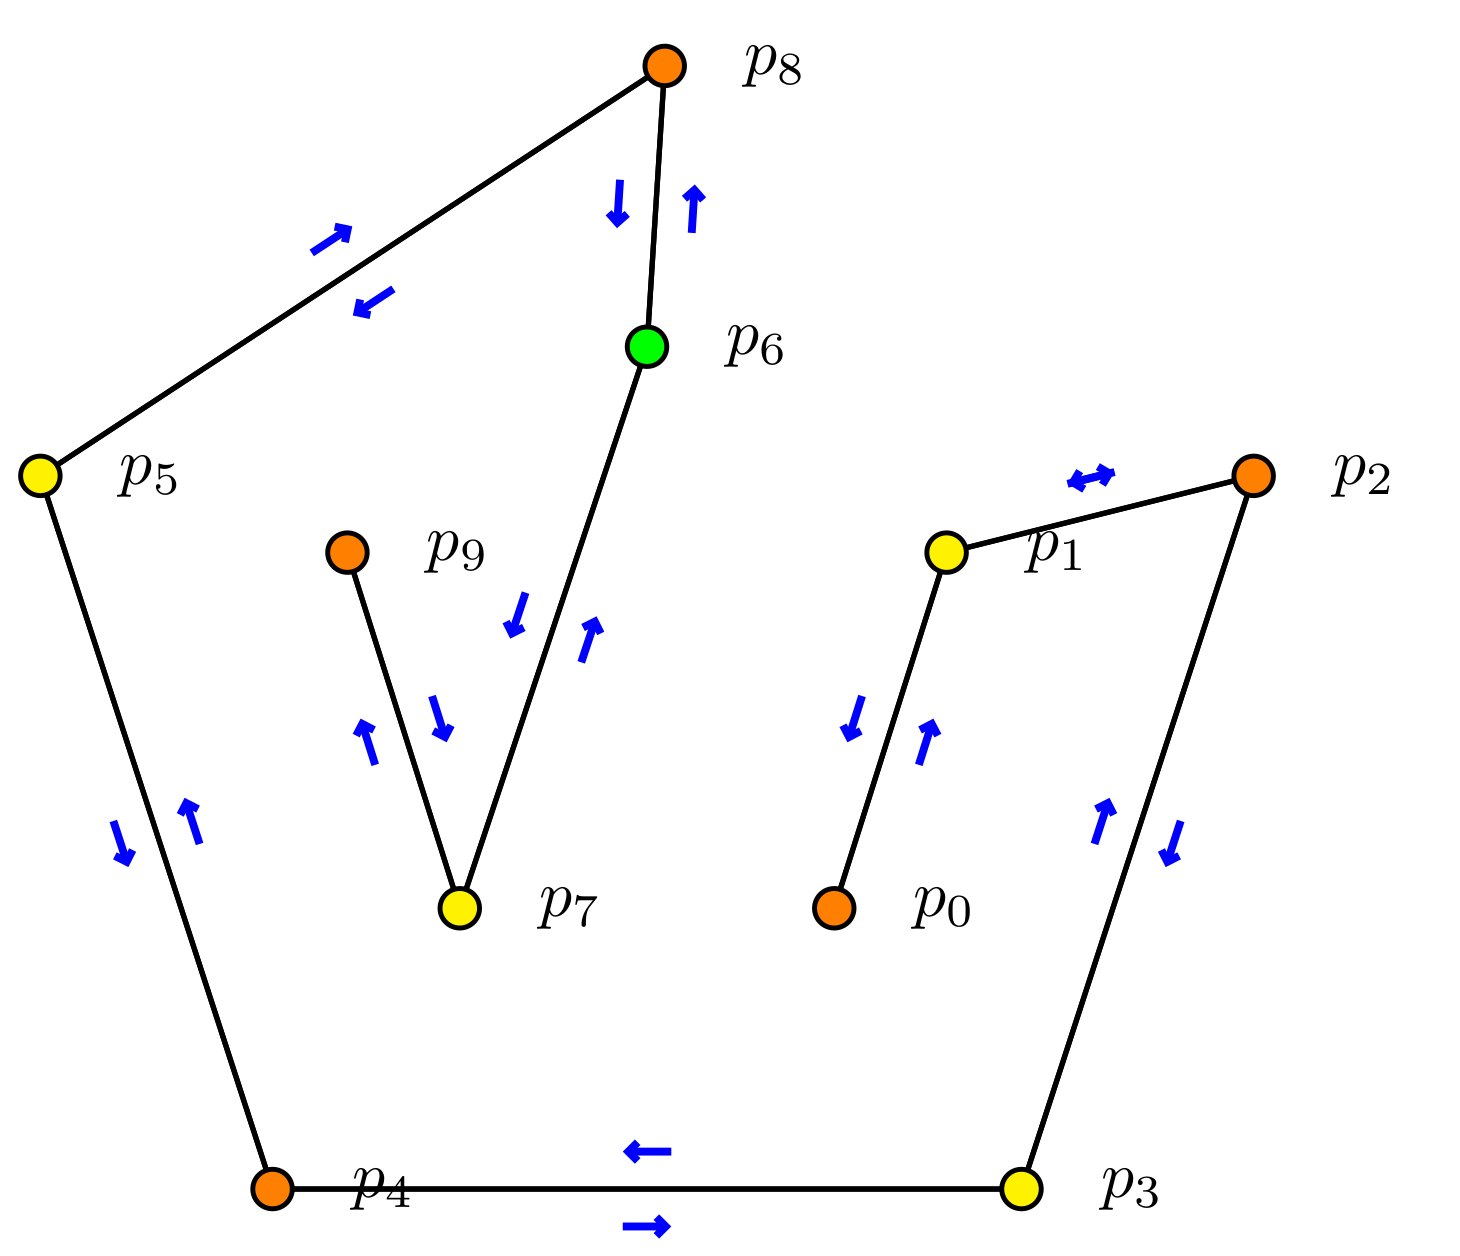
\includegraphics[width=7cm]{RD7.png}
                \caption{Gŕagica correspondiente a $R_7$.}
        \end{center}
\end{figure}

En la ronda 8 tenemos que:

\begin{multicols}{2}
\begin{itemize}
\item Estado de $p_0$:
      \begin{itemize}
      %%%%%%%%%%%%%%%% M
      \item \code{M = $\{\langle ID_1, 2 \rangle\}$}
      
      %%%%%%%%%%%%%%%% A
      \item \code{A = $\emptyset$}
      
      %%%%%%%%%%%%%%%% C
      \item \code{C = $1$}
      \end{itemize}
      
\item Estado de $p_1$:
      \begin{itemize}
      %%%%%%%%%%%%%%%% M
      \item \code{M = $\{\langle ID_0, 1 \rangle,\;
                         \langle ID_2, 1 \rangle\}$}
      
      %%%%%%%%%%%%%%%% A
      \item \code{A = $\emptyset$}
      
      %%%%%%%%%%%%%%%% C
      \item \code{C = $2$}
      \end{itemize}

\item Estado de $p_2$:
      \begin{itemize}
      %%%%%%%%%%%%%%%% M
      \item \code{M = $\{\langle ID_1, 2 \rangle,\;
                         \langle ID_3, 2 \rangle\}$}
      
      %%%%%%%%%%%%%%%% A
      \item \code{A = $\emptyset$}
      
      %%%%%%%%%%%%%%%% C
      \item \code{C = $1$}
      \end{itemize}

\item Estado de $p_3$:
      \begin{itemize}
      %%%%%%%%%%%%%%%% M
      \item \code{M = $\{\langle ID_2, 1 \rangle,\;
                         \langle ID_4, 1 \rangle\}$}
      
      %%%%%%%%%%%%%%%% A
      \item \code{A = $\emptyset$}
      
      %%%%%%%%%%%%%%%% C
      \item \code{C = $2$}
      \end{itemize}

\item Estado de $p_4$:
      \begin{itemize}
      %%%%%%%%%%%%%%%% M
      \item \code{M = $\{\langle ID_3, 2 \rangle,\;
                         \langle ID_5, 2 \rangle\}$}
      
      %%%%%%%%%%%%%%%% A
      \item \code{A = $\emptyset$}
      
      %%%%%%%%%%%%%%%% C
      \item \code{C = $1$}
      \end{itemize}

\item Estado de $p_5$:
      \begin{itemize}
      %%%%%%%%%%%%%%%% M
      \item \code{M = $\{\langle ID_4, 1 \rangle,\;
                         \langle ID_8, 1 \rangle\}$}
      
      %%%%%%%%%%%%%%%% A
      \item \code{A = $\emptyset$}
      
      %%%%%%%%%%%%%%%% C
      \item \code{C = $1$}
      \end{itemize}

\item Estado de $p_6$:
      \begin{itemize}
      %%%%%%%%%%%%%%%% M
      \item \code{M = $\{\langle ID_7, 2 \rangle,\;
                         \langle ID_8, 1 \rangle\}$}
      
      %%%%%%%%%%%%%%%% A
      \item \code{A = $\emptyset$}
      
      %%%%%%%%%%%%%%%% C
      \item \code{C = $3$}
      \end{itemize}

\item Estado de $p_7$:
      \begin{itemize}
      %%%%%%%%%%%%%%%% M
      \item \code{M = $\{\langle ID_6, 3 \rangle,\;
                         \langle ID_9, 1 \rangle\}$}
      
      %%%%%%%%%%%%%%%% A
      \item \code{A = $\emptyset$}
      
      %%%%%%%%%%%%%%%% C
      \item \code{C = $2$}
      \end{itemize}

\item Estado de $p_8$:
      \begin{itemize}
      %%%%%%%%%%%%%%%% M
      \item \code{M = $\{\langle ID_5, 2 \rangle,\;
                         \langle ID_6, 3 \rangle\}$}
      
      %%%%%%%%%%%%%%%% A
      \item \code{A = $\emptyset$}
      
      %%%%%%%%%%%%%%%% C
      \item \code{C = $1$}
      \end{itemize}

\item Estado de $p_9$:
      \begin{itemize}
      %%%%%%%%%%%%%%%% M
      \item \code{M = $\{\langle ID_7, 2 \rangle\}$}
      
      %%%%%%%%%%%%%%%% A
      \item \code{A = $\emptyset$}
      
      %%%%%%%%%%%%%%%% C
      \item \code{C = $1$}
      \end{itemize}

\end{itemize}
\end{multicols} 

Como podemos notar, en la ronda $8$ ($R_8$) no se colorea ningún proceso,
pues todos han sido coloreados. En esta ronda solo hacemos $A = \emptyset$
a los procesos restantes. La complejidad en tiempo del algoritmo ha sido
\begin{center}
        \code{diam($G$) $- 2$} $\in \mathcal{O}(\code{diam(G)})$.
\end{center}
\newpage

\hspace*{0.5cm} \textbf{\textcolor{blue}{2}}. Mostrar una ejecución
en tiempo $\frac{\code{diam($G$)}}{2}$, con $G$ una gráfica tal que $|V_G| = 10$.
La nueva asignación de $ID_i$'s se muestra a continuación:

\begin{figure}[ht!]
     \centering
     \begin{tikzpicture}
        \begin{scope}
           % Fig exterior:
           \node(0) [vertex, label=180:$p_0$] at (0, 6)        {};
           \node(1) [vertex, label=360:$p_1$] at (3.24, 3.81)  {};
           \node(2) [vertex, label=360:$p_2$] at (2,  0)       {};
           \node(3) [vertex, label=180:$p_3$] at (-2, 0)       {};
           \node(4) [vertex, label=180:$p_4$] at (-3.24, 3.81) {};
           % Fig interior:
           \node(5) [vertex, label=180:$p_5$] at (0, 4.5)      {};
           \node(6) [vertex, label=180:$p_6$] at (1.6,  3.4)   {};
           \node(7) [vertex, label=180:$p_7$] at (1, 1.5)      {};
           \node(8) [vertex, label=180:$p_8$] at (-1, 1.5)     {};
           \node(9) [vertex, label=180:$p_9$] at (-1.6, 3.4)   {};
           
           % Segmentos
           \draw [edge] (1) to (2);
           \draw [edge] (2) to (3);
           \draw [edge] (3) to (4);
           \draw [edge] (4) to (0);
           \draw [edge] (0) to (5);
           \draw [edge] (1) to (6);
           \draw [edge] (5) to (8);
           \draw [edge] (6) to (7);
           \draw [edge] (9) to (8);
           
           \node (L) at (-3,6){$G$};
        \end{scope}
     \end{tikzpicture}
\caption{Gŕagica $G$.}
\label{fig:fam1}
\end{figure}

En la ronda 0 tenemos que: \newline

Se envían los $ID_i$'s a todos los vecinos para cada proceso, por
motivos de visualización de la gráfica no se ilustra cada $ID_i$
para algún $i \in [0, \dotsm, 9]$, pero cuándo sea necesario se
indicara \footnote{Además es claro que para un proceso $p_j$ existe
un $ID_j$ único.}. 

\begin{figure}[ht]
        \begin{center}
                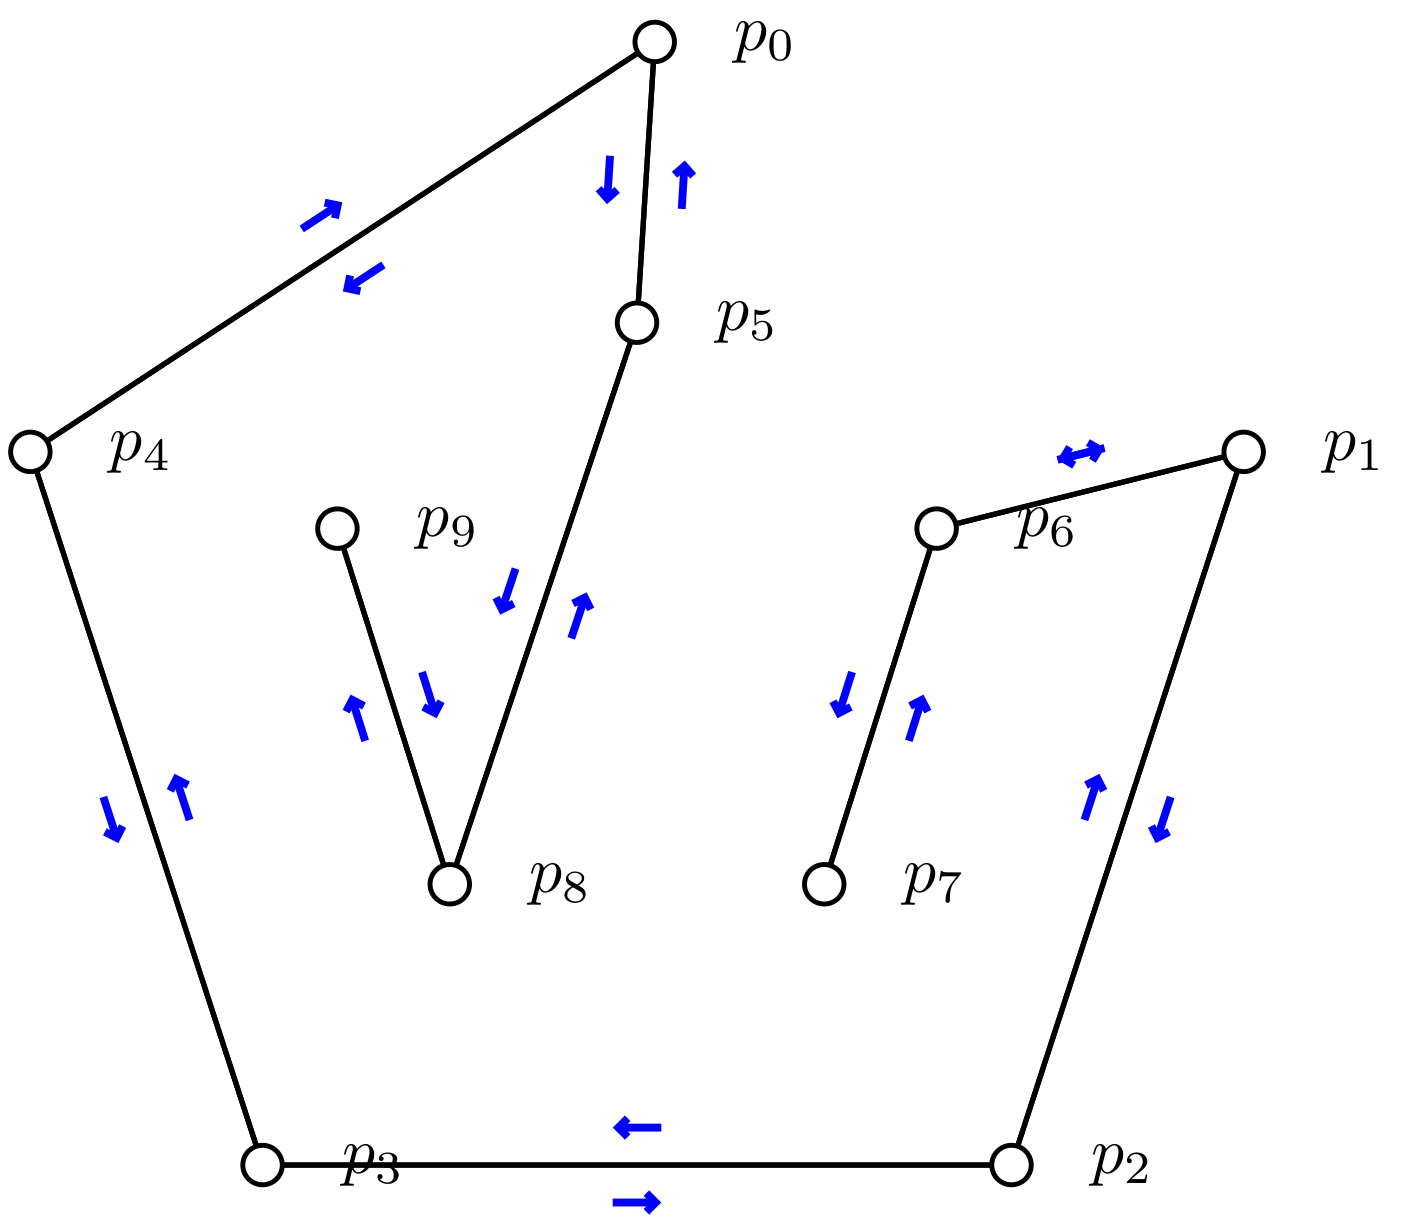
\includegraphics[width=7cm]{R0.png}
                \caption{Gŕagica correspondiente a $R_0$.}
        \end{center}
\end{figure}

En la ronda 1 tenemos que:

\begin{multicols}{2}
\begin{itemize}
\item Estado de $p_0$:
      \begin{itemize}
      %%%%%%%%%%%%%%%% M
      \item \code{M = $\{\langle ID_4, \bot \rangle,\;
                         \langle ID_5, \bot \rangle\}$}
      
      %%%%%%%%%%%%%%%% A
      \item \code{A = $\{ID_4,\; ID_5\}$}
      
      %%%%%%%%%%%%%%%% C
      \item \code{C = $\bot$}
      \end{itemize}
      
\item Estado de $p_1$:
      \begin{itemize}
      %%%%%%%%%%%%%%%% M
      \item \code{M = $\{\langle ID_2, \bot \rangle,\;
                         \langle ID_6, \bot \rangle\}$}
      
      %%%%%%%%%%%%%%%% A
      \item \code{A = $\{ID_2,\; ID_6\}$}
      
      %%%%%%%%%%%%%%%% C
      \item \code{C = $\bot$}
      \end{itemize}

\item Estado de $p_2$:
      \begin{itemize}
      %%%%%%%%%%%%%%%% M
      \item \code{M = $\{\langle ID_1, \bot \rangle,\;
                         \langle ID_3, \bot \rangle\}$}
      
      %%%%%%%%%%%%%%%% A
      \item \code{A = $\{ID_1,\; ID_3\}$}
      
      %%%%%%%%%%%%%%%% C
      \item \code{C = $\bot$}
      \end{itemize}

\item Estado de $p_3$:
      \begin{itemize}
      %%%%%%%%%%%%%%%% M
      \item \code{M = $\{\langle ID_2, \bot \rangle,\;
                         \langle ID_4, \bot \rangle\}$}
      
      %%%%%%%%%%%%%%%% A
      \item \code{A = $\{ID_2,\; ID_4\}$}
      
      %%%%%%%%%%%%%%%% C
      \item \code{C = $\bot$}
      \end{itemize}

\item Estado de $p_4$:
      \begin{itemize}
      %%%%%%%%%%%%%%%% M
      \item \code{M = $\{\langle ID_0, \bot \rangle,\;
                         \langle ID_3, \bot \rangle\}$}
      
      %%%%%%%%%%%%%%%% A
      \item \code{A = $\{ID_0,\; ID_3\}$}
      
      %%%%%%%%%%%%%%%% C
      \item \code{C = $1$}
      \end{itemize}

\item Estado de $p_5$:
      \begin{itemize}
      %%%%%%%%%%%%%%%% M
      \item \code{M = $\{\langle ID_0, \bot \rangle,\;
                         \langle ID_8, \bot \rangle\}$}
      
      %%%%%%%%%%%%%%%% A
      \item \code{A = $\{ID_0,\; ID_8\}$}
      
      %%%%%%%%%%%%%%%% C
      \item \code{C = $\bot$}
      \end{itemize}

\item Estado de $p_6$:
      \begin{itemize}
      %%%%%%%%%%%%%%%% M
      \item \code{M = $\{\langle ID_1, \bot \rangle,\;
                         \langle ID_7, \bot \rangle\}$}
      
      %%%%%%%%%%%%%%%% A
      \item \code{A = $\{ID_1,\; ID_7\}$}
      
      %%%%%%%%%%%%%%%% C
      \item \code{C = $\bot$}
      \end{itemize}

\item Estado de $p_7$:
      \begin{itemize}
      %%%%%%%%%%%%%%%% M
      \item \code{M = $\{\langle ID_6, \bot \rangle\}$}
      
      %%%%%%%%%%%%%%%% A
      \item \code{A = $\{ID_6\}$}
      
      %%%%%%%%%%%%%%%% C
      \item \code{C = $1$}
      \end{itemize}

\item Estado de $p_8$:
      \begin{itemize}
      %%%%%%%%%%%%%%%% M
      \item \code{M = $\{\langle ID_5, \bot \rangle,\;
                         \langle ID_9, \bot \rangle\}$}
      
      %%%%%%%%%%%%%%%% A
      \item \code{A = $\{ID_5,\; ID_9\}$}
      
      %%%%%%%%%%%%%%%% C
      \item \code{C = $\bot$}
      \end{itemize}

\item Estado de $p_9$:
      \begin{itemize}
      %%%%%%%%%%%%%%%% M
      \item \code{M = $\{\langle ID_8, \bot \rangle\}$}
      
      %%%%%%%%%%%%%%%% A
      \item \code{A = $\{ID_8\}$}
      
      %%%%%%%%%%%%%%%% C
      \item \code{C = $1$}
      \end{itemize}

\end{itemize}
\end{multicols} 

\begin{figure}[ht]
        \begin{center}
                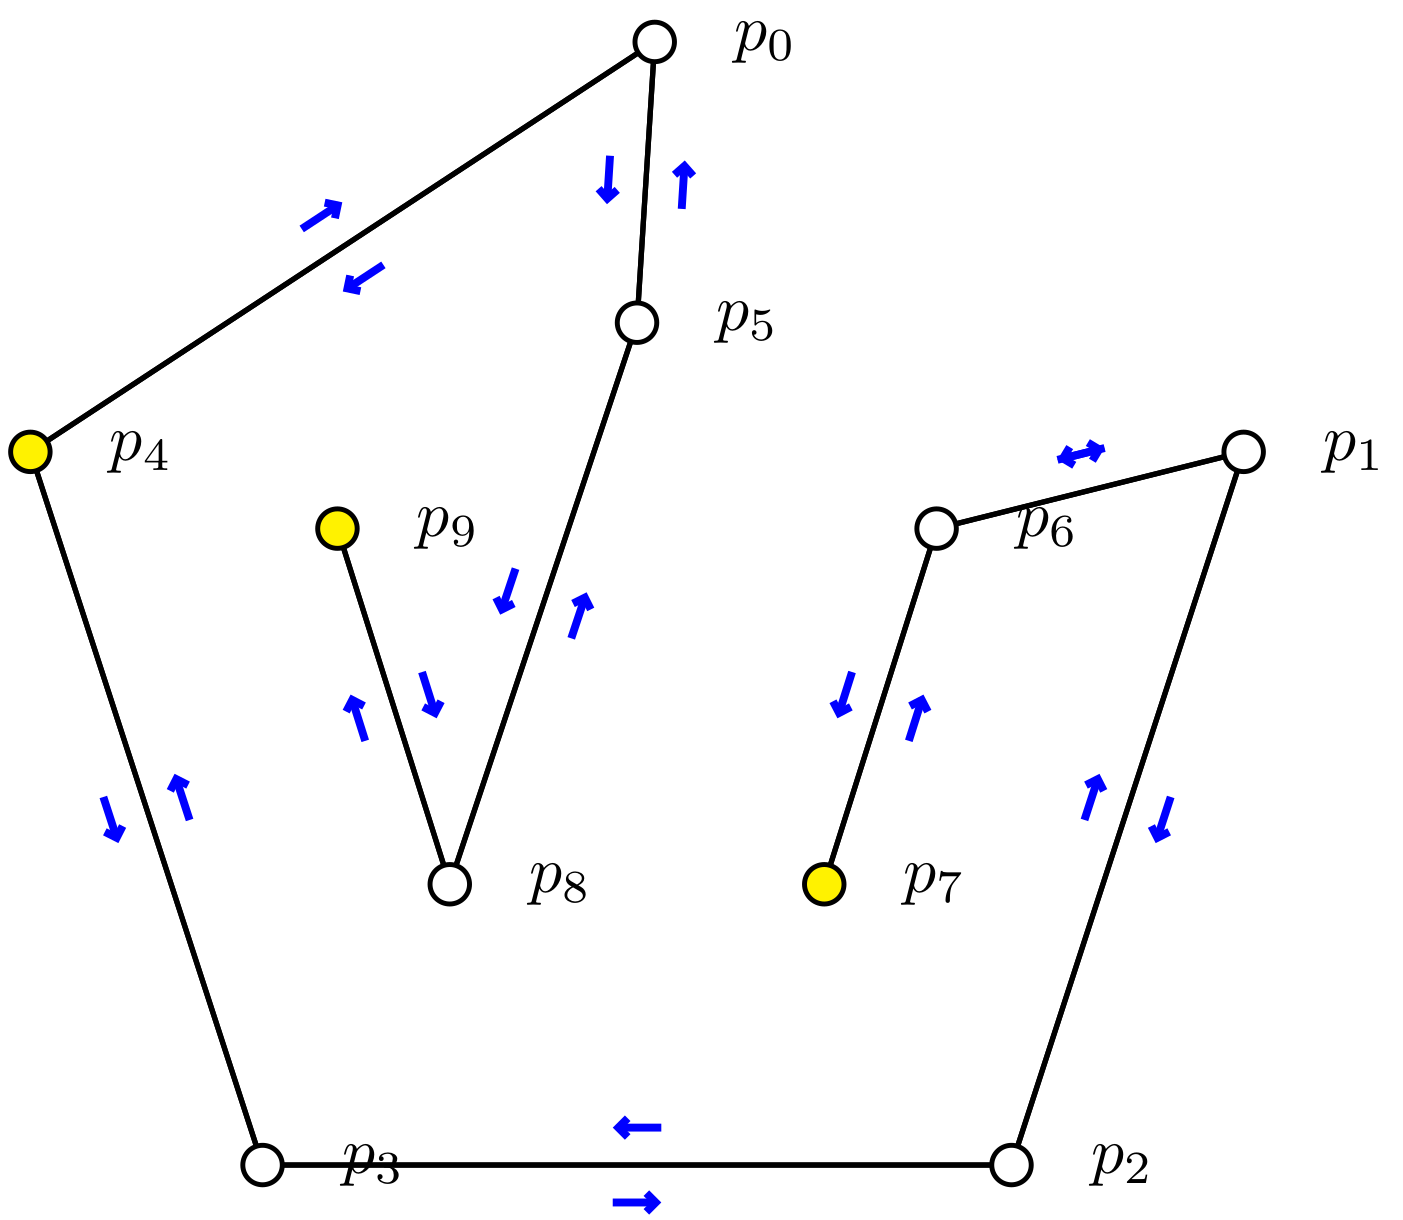
\includegraphics[width=7cm]{R1.png}
                \caption{Gŕagica correspondiente a $R_1$.}
        \end{center}
\end{figure}

En la ronda 2 tenemos que:
\begin{multicols}{2}
\begin{itemize}
\item Estado de $p_0$:
      \begin{itemize}
      %%%%%%%%%%%%%%%% M
      \item \code{M = $\{\langle ID_4, 1 \rangle,\;
                         \langle ID_5, \bot \rangle\}$}
      
      %%%%%%%%%%%%%%%% A
      \item \code{A = $\{ID_5\}$}
      
      %%%%%%%%%%%%%%%% C
      \item \code{C = $\bot$}
      \end{itemize}
      
\item Estado de $p_1$:
      \begin{itemize}
      %%%%%%%%%%%%%%%% M
      \item \code{M = $\{\langle ID_2, \bot \rangle,\;
                         \langle ID_6, \bot \rangle\}$}
      
      %%%%%%%%%%%%%%%% A
      \item \code{A = $\{ID_2,\; ID_6\}$}
      
      %%%%%%%%%%%%%%%% C
      \item \code{C = $\bot$}
      \end{itemize}

\item Estado de $p_2$:
      \begin{itemize}
      %%%%%%%%%%%%%%%% M
      \item \code{M = $\{\langle ID_1, \bot \rangle,\;
                         \langle ID_3, \bot \rangle\}$}
      
      %%%%%%%%%%%%%%%% A
      \item \code{A = $\{ID_1,\; ID_3\}$}
      
      %%%%%%%%%%%%%%%% C
      \item \code{C = $\bot$}
      \end{itemize}

\item Estado de $p_3$:
      \begin{itemize}
      %%%%%%%%%%%%%%%% M
      \item \code{M = $\{\langle ID_2, \bot \rangle,\;
                         \langle ID_4, 1 \rangle\}$}
      
      %%%%%%%%%%%%%%%% A
      \item \code{A = $\{ID_2\}$}
      
      %%%%%%%%%%%%%%%% C
      \item \code{C = $2$}
      \end{itemize}

\item Estado de $p_4$:
      \begin{itemize}
      %%%%%%%%%%%%%%%% M
      \item \code{M = $\{\langle ID_0, \bot \rangle,\;
                         \langle ID_3, \bot \rangle\}$}
      
      %%%%%%%%%%%%%%%% A
      \item \code{A = $\{ID_0,\; ID_3\}$}
      
      %%%%%%%%%%%%%%%% C
      \item \code{C = $1$}
      \end{itemize}

\item Estado de $p_5$:
      \begin{itemize}
      %%%%%%%%%%%%%%%% M
      \item \code{M = $\{\langle ID_0, \bot \rangle,\;
                         \langle ID_8, \bot \rangle\}$}
      
      %%%%%%%%%%%%%%%% A
      \item \code{A = $\{ID_0,\; ID_8\}$}
      
      %%%%%%%%%%%%%%%% C
      \item \code{C = $\bot$}
      \end{itemize}

\item Estado de $p_6$:
      \begin{itemize}
      %%%%%%%%%%%%%%%% M
      \item \code{M = $\{\langle ID_1, \bot \rangle,\;
                         \langle ID_7, 1 \rangle\}$}
      
      %%%%%%%%%%%%%%%% A
      \item \code{A = $\{ID_1\}$}
      
      %%%%%%%%%%%%%%%% C
      \item \code{C = $2$}
      \end{itemize}

\item Estado de $p_7$:
      \begin{itemize}
      %%%%%%%%%%%%%%%% M
      \item \code{M = $\{\langle ID_6, \bot \rangle\}$}
      
      %%%%%%%%%%%%%%%% A
      \item \code{A = $\{ID_6\}$}
      
      %%%%%%%%%%%%%%%% C
      \item \code{C = $1$}
      \end{itemize}

\item Estado de $p_8$:
      \begin{itemize}
      %%%%%%%%%%%%%%%% M
      \item \code{M = $\{\langle ID_5, \bot \rangle,\;
                         \langle ID_9, 1 \rangle\}$}
      
      %%%%%%%%%%%%%%%% A
      \item \code{A = $\{ID_5\}$}
      
      %%%%%%%%%%%%%%%% C
      \item \code{C = $2$}
      \end{itemize}

\item Estado de $p_9$:
      \begin{itemize}
      %%%%%%%%%%%%%%%% M
      \item \code{M = $\{\langle ID_8, \bot \rangle\}$}
      
      %%%%%%%%%%%%%%%% A
      \item \code{A = $\{ID_8\}$}
      
      %%%%%%%%%%%%%%%% C
      \item \code{C = $1$}
      \end{itemize}

\end{itemize}
\end{multicols} 

\begin{figure}[ht]
        \begin{center}
                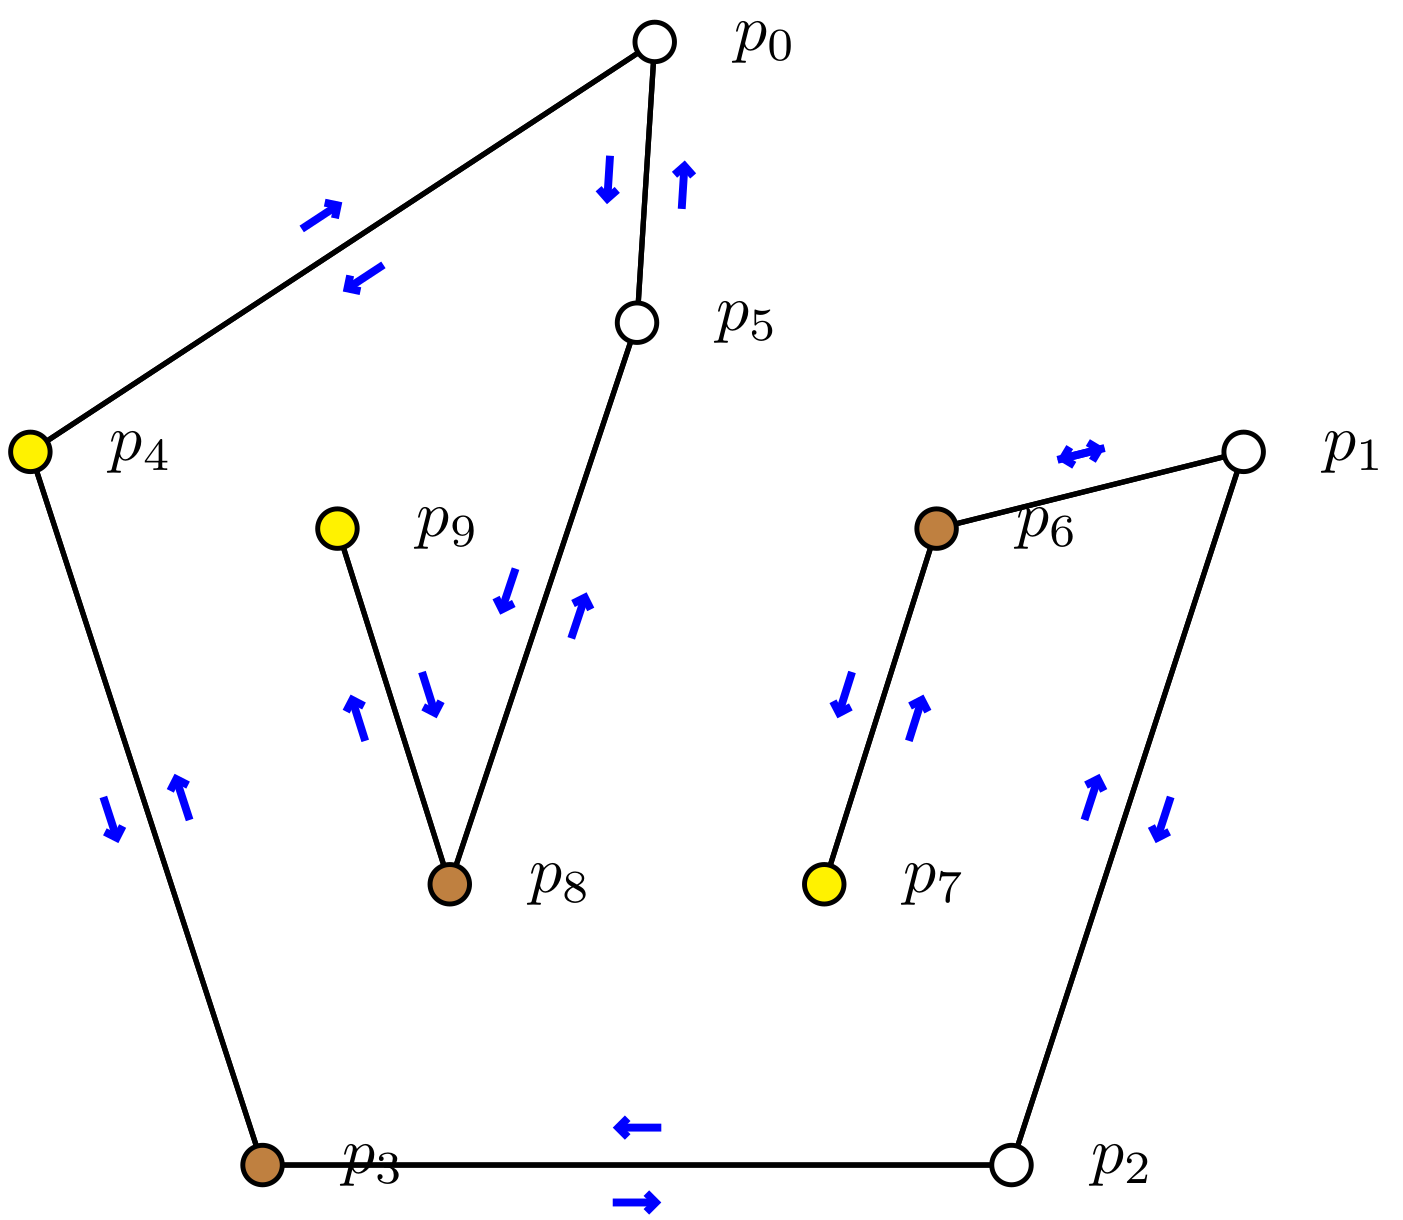
\includegraphics[width=7cm]{R2.png}
                \caption{Gŕagica correspondiente a $R_2$.}
        \end{center}
\end{figure}

En la ronda 3 tenemos que:
\begin{multicols}{2}
\begin{itemize}
\item Estado de $p_0$:
      \begin{itemize}
      %%%%%%%%%%%%%%%% M
      \item \code{M = $\{\langle ID_4, 1 \rangle,\;
                         \langle ID_5, \bot \rangle\}$}
      
      %%%%%%%%%%%%%%%% A
      \item \code{A = $\{ID_5\}$}
      
      %%%%%%%%%%%%%%%% C
      \item \code{C = $\bot$}
      \end{itemize}
      
\item Estado de $p_1$:
      \begin{itemize}
      %%%%%%%%%%%%%%%% M
      \item \code{M = $\{\langle ID_2, \bot \rangle,\;
                         \langle ID_6, \bot \rangle\}$}
      
      %%%%%%%%%%%%%%%% A
      \item \code{A = $\{ID_2,\; ID_6\}$}
      
      %%%%%%%%%%%%%%%% C
      \item \code{C = $\bot$}
      \end{itemize}

\item Estado de $p_2$:
      \begin{itemize}
      %%%%%%%%%%%%%%%% M
      \item \code{M = $\{\langle ID_1, \bot \rangle,\;
                         \langle ID_3, 2 \rangle\}$}
      
      %%%%%%%%%%%%%%%% A
      \item \code{A = $\{ID_1\}$}
      
      %%%%%%%%%%%%%%%% C
      \item \code{C = $1$}
      \end{itemize}

\item Estado de $p_3$:
      \begin{itemize}
      %%%%%%%%%%%%%%%% M
      \item \code{M = $\{\langle ID_2, \bot \rangle,\;
                         \langle ID_4, 1 \rangle\}$}
      
      %%%%%%%%%%%%%%%% A
      \item \code{A = $\{ID_2\}$}
      
      %%%%%%%%%%%%%%%% C
      \item \code{C = $2$}
      \end{itemize}

\item Estado de $p_4$:
      \begin{itemize}
      %%%%%%%%%%%%%%%% M
      \item \code{M = $\{\langle ID_0, \bot \rangle,\;
                         \langle ID_3, \bot \rangle\}$}
      
      %%%%%%%%%%%%%%%% A
      \item \code{A = $\{ID_0,\; ID_3\}$}
      
      %%%%%%%%%%%%%%%% C
      \item \code{C = $1$}
      \end{itemize}

\item Estado de $p_5$:
      \begin{itemize}
      %%%%%%%%%%%%%%%% M
      \item \code{M = $\{\langle ID_0, \bot \rangle,\;
                         \langle ID_8, 2 \rangle\}$}
      
      %%%%%%%%%%%%%%%% A
      \item \code{A = $\{ID_0\}$}
      
      %%%%%%%%%%%%%%%% C
      \item \code{C = $1$}
      \end{itemize}

\item Estado de $p_6$:
      \begin{itemize}
      %%%%%%%%%%%%%%%% M
      \item \code{M = $\{\langle ID_1, \bot \rangle,\;
                         \langle ID_7, 1 \rangle\}$}
      
      %%%%%%%%%%%%%%%% A
      \item \code{A = $\{ID_1\}$}
      
      %%%%%%%%%%%%%%%% C
      \item \code{C = $2$}
      \end{itemize}

\item Estado de $p_7$:
      \begin{itemize}
      %%%%%%%%%%%%%%%% M
      \item \code{M = $\{\langle ID_6, 2 \rangle\}$}
      
      %%%%%%%%%%%%%%%% A
      \item \code{A = $\emptyset$}
      
      %%%%%%%%%%%%%%%% C
      \item \code{C = $1$}
      \end{itemize}

\item Estado de $p_8$:
      \begin{itemize}
      %%%%%%%%%%%%%%%% M
      \item \code{M = $\{\langle ID_5, \bot \rangle,\;
                         \langle ID_9, 1 \rangle\}$}
      
      %%%%%%%%%%%%%%%% A
      \item \code{A = $\{ID_5\}$}
      
      %%%%%%%%%%%%%%%% C
      \item \code{C = $2$}
      \end{itemize}

\item Estado de $p_9$:
      \begin{itemize}
      %%%%%%%%%%%%%%%% M
      \item \code{M = $\{\langle ID_8, 2 \rangle\}$}
      
      %%%%%%%%%%%%%%%% A
      \item \code{A = $\emptyset$}
      
      %%%%%%%%%%%%%%%% C
      \item \code{C = $1$}
      \end{itemize}

\end{itemize}
\end{multicols} 

\begin{figure}[ht]
        \begin{center}
                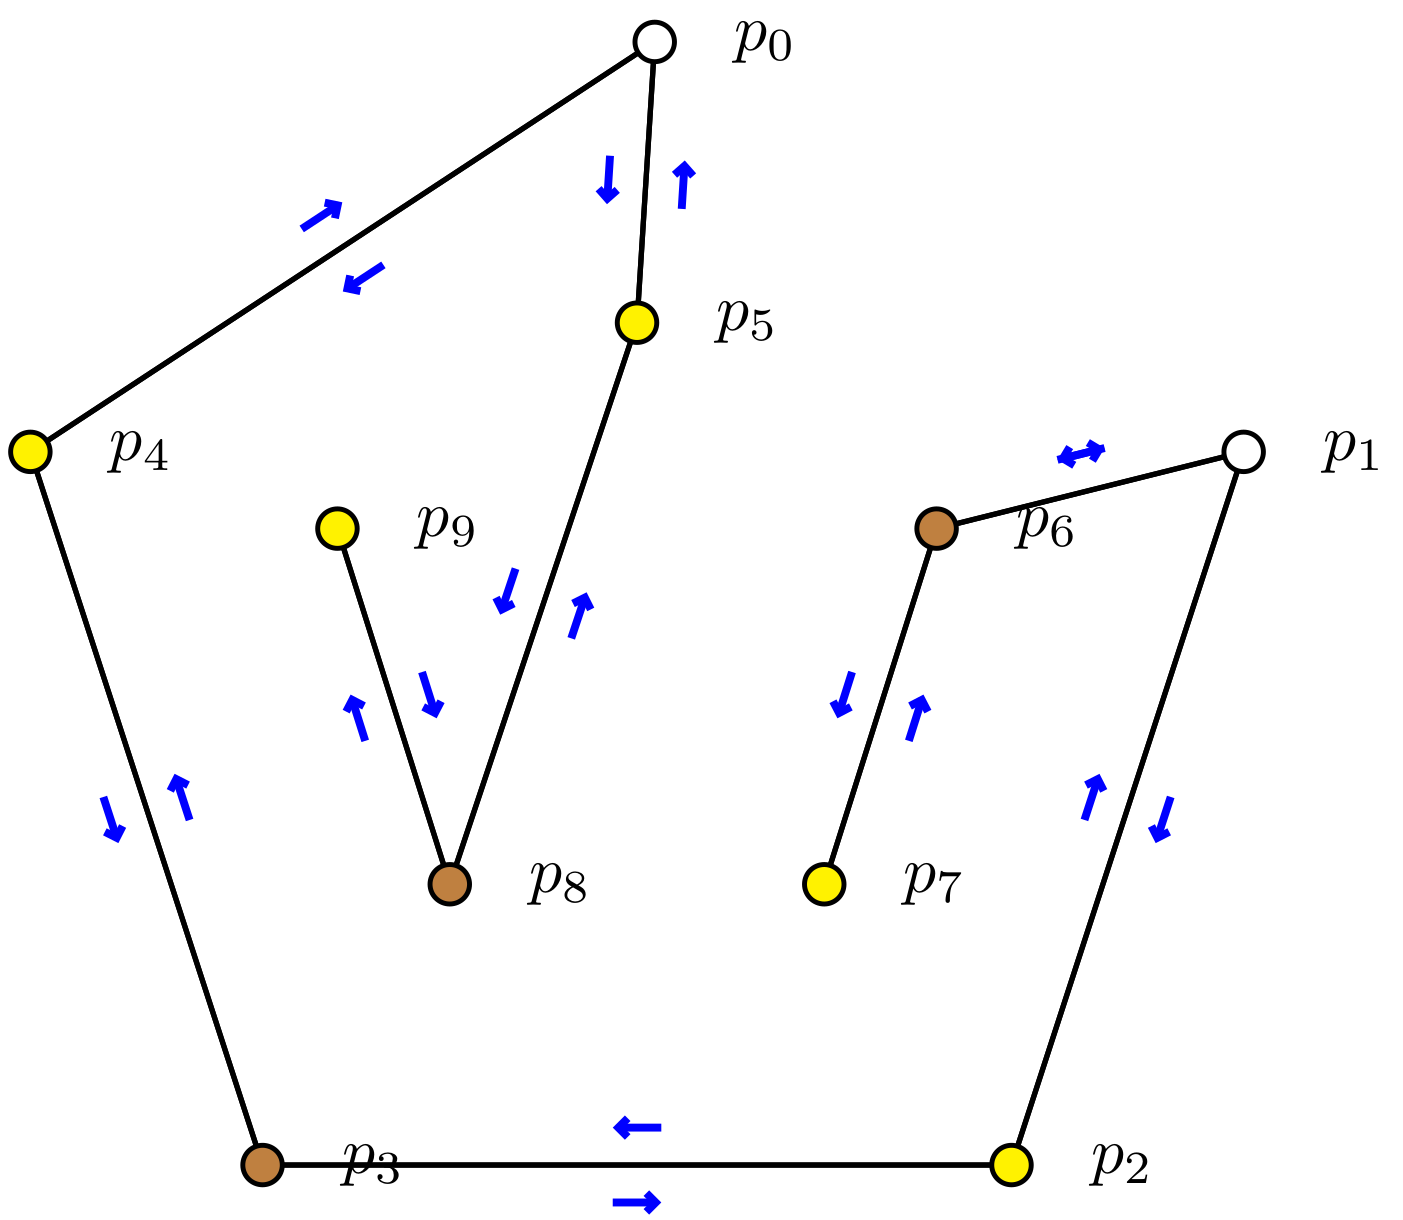
\includegraphics[width=7cm]{R3.png}
                \caption{Gŕagica correspondiente a $R_3$.}
        \end{center}
\end{figure}

En la ronda 4 tenemos que:
\begin{multicols}{2}
\begin{itemize}
\item Estado de $p_0$:
      \begin{itemize}
      %%%%%%%%%%%%%%%% M
      \item \code{M = $\{\langle ID_4, 1 \rangle,\;
                         \langle ID_5, 1 \rangle\}$}
      
      %%%%%%%%%%%%%%%% A
      \item \code{A = $\emptyset$}
      
      %%%%%%%%%%%%%%%% C
      \item \code{C = $2$}
      \end{itemize}
      
\item Estado de $p_1$:
      \begin{itemize}
      %%%%%%%%%%%%%%%% M
      \item \code{M = $\{\langle ID_2, 1 \rangle,\;
                         \langle ID_6, 2 \rangle\}$}
      
      %%%%%%%%%%%%%%%% A
      \item \code{A = $\emptyset$}
      
      %%%%%%%%%%%%%%%% C
      \item \code{C = $3$}
      \end{itemize}

\item Estado de $p_2$:
      \begin{itemize}
      %%%%%%%%%%%%%%%% M
      \item \code{M = $\{\langle ID_1, \bot \rangle,\;
                         \langle ID_3, 2 \rangle\}$}
      
      %%%%%%%%%%%%%%%% A
      \item \code{A = $\{ID_1\}$}
      
      %%%%%%%%%%%%%%%% C
      \item \code{C = $1$}
      \end{itemize}

\item Estado de $p_3$:
      \begin{itemize}
      %%%%%%%%%%%%%%%% M
      \item \code{M = $\{\langle ID_2, 1 \rangle,\;
                         \langle ID_4, 1 \rangle\}$}
      
      %%%%%%%%%%%%%%%% A
      \item \code{A = $\emptyset$}
      
      %%%%%%%%%%%%%%%% C
      \item \code{C = $2$}
      \end{itemize}

\item Estado de $p_4$:
      \begin{itemize}
      %%%%%%%%%%%%%%%% M
      \item \code{M = $\{\langle ID_0, \bot \rangle,\;
                         \langle ID_3, 2 \rangle\}$}
      
      %%%%%%%%%%%%%%%% A
      \item \code{A = $\{ID_0\}$}
      
      %%%%%%%%%%%%%%%% C
      \item \code{C = $1$}
      \end{itemize}

\item Estado de $p_5$:
      \begin{itemize}
      %%%%%%%%%%%%%%%% M
      \item \code{M = $\{\langle ID_0, \bot \rangle,\;
                         \langle ID_8, 2 \rangle\}$}
      
      %%%%%%%%%%%%%%%% A
      \item \code{A = $\{ID_0\}$}
      
      %%%%%%%%%%%%%%%% C
      \item \code{C = $1$}
      \end{itemize}

\item Estado de $p_6$:
      \begin{itemize}
      %%%%%%%%%%%%%%%% M
      \item \code{M = $\{\langle ID_1, \bot \rangle,\;
                         \langle ID_7, 1 \rangle\}$}
      
      %%%%%%%%%%%%%%%% A
      \item \code{A = $\{ID_1\}$}
      
      %%%%%%%%%%%%%%%% C
      \item \code{C = $2$}
      \end{itemize}

\item Estado de $p_7$:
      \begin{itemize}
      %%%%%%%%%%%%%%%% M
      \item \code{M = $\{\langle ID_6, 2 \rangle\}$}
      
      %%%%%%%%%%%%%%%% A
      \item \code{A = $\emptyset$}
      
      %%%%%%%%%%%%%%%% C
      \item \code{C = $1$}
      \end{itemize}

\item Estado de $p_8$:
      \begin{itemize}
      %%%%%%%%%%%%%%%% M
      \item \code{M = $\{\langle ID_5, 1 \rangle,\;
                         \langle ID_9, 1 \rangle\}$}
      
      %%%%%%%%%%%%%%%% A
      \item \code{A = $\emptyset$}
      
      %%%%%%%%%%%%%%%% C
      \item \code{C = $2$}
      \end{itemize}

\item Estado de $p_9$:
      \begin{itemize}
      %%%%%%%%%%%%%%%% M
      \item \code{M = $\{\langle ID_8, 2 \rangle\}$}
      
      %%%%%%%%%%%%%%%% A
      \item \code{A = $\emptyset$}
      
      %%%%%%%%%%%%%%%% C
      \item \code{C = $1$}
      \end{itemize}

\end{itemize}
\end{multicols} 

\begin{figure}[ht]
        \begin{center}
                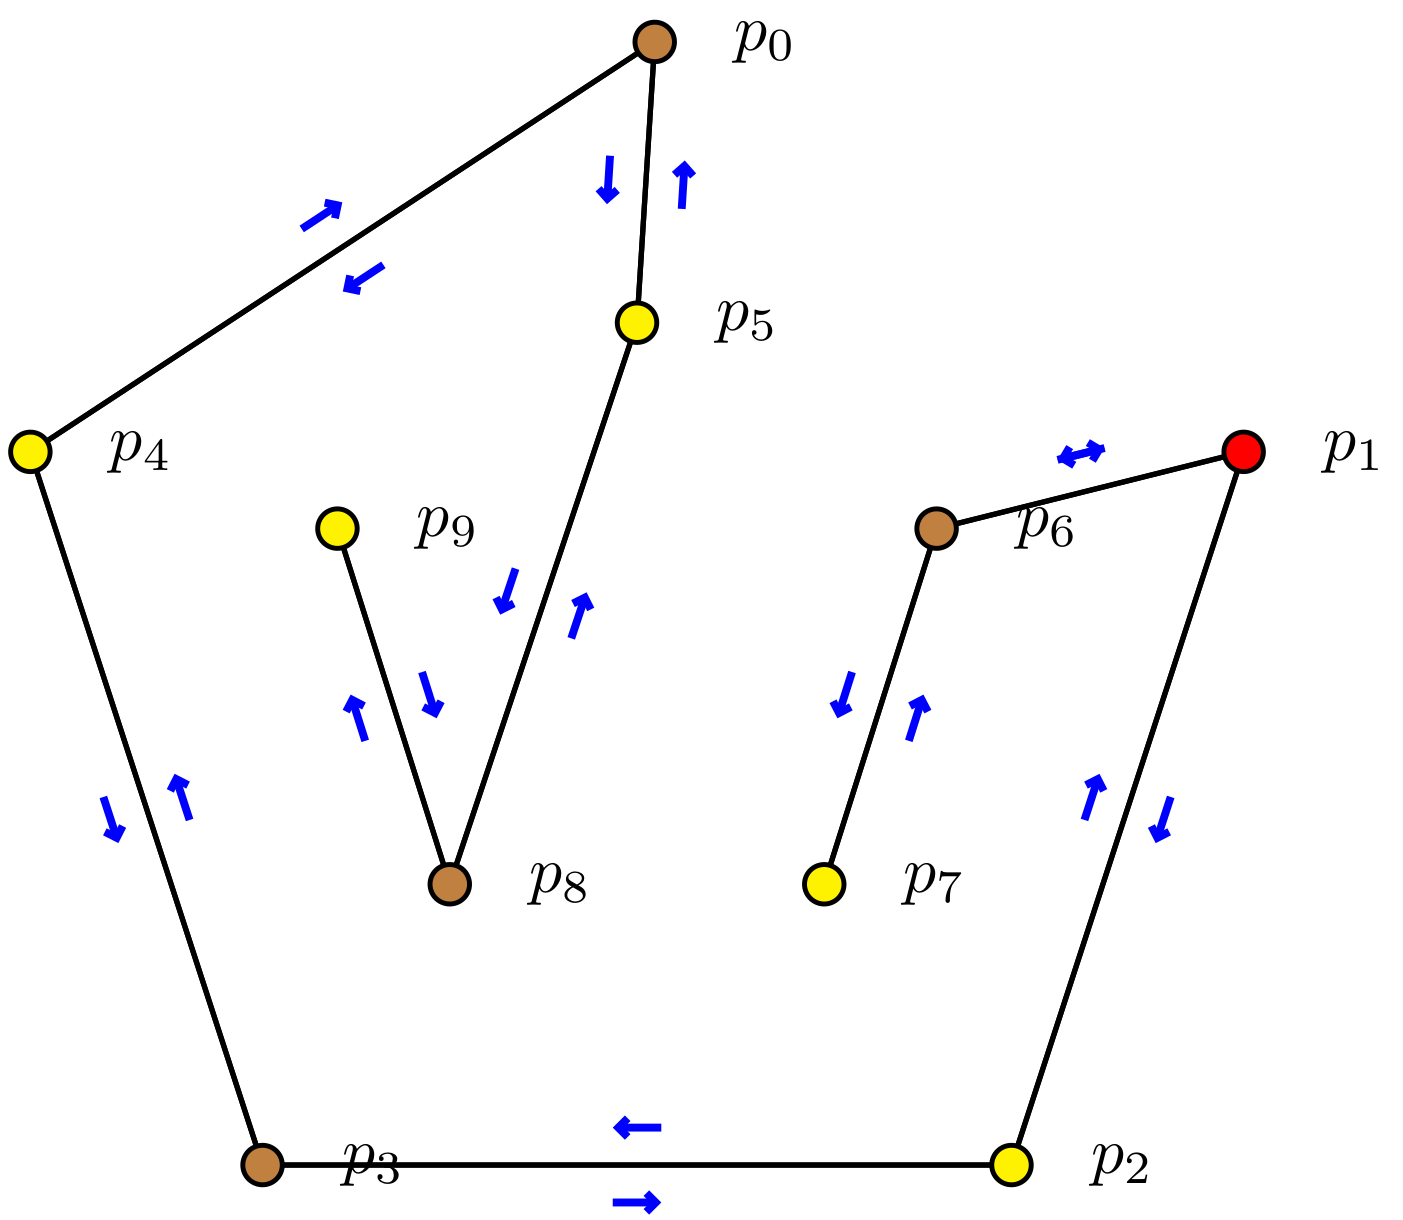
\includegraphics[width=7cm]{R4.png}
                \caption{Gŕagica correspondiente a $R_4$.}
        \end{center}
\end{figure}

En la ronda 5 tenemos que:
\begin{multicols}{2}
\begin{itemize}
\item Estado de $p_0$:
      \begin{itemize}
      %%%%%%%%%%%%%%%% M
      \item \code{M = $\{\langle ID_4, 1 \rangle,\;
                         \langle ID_5, 1 \rangle\}$}
      
      %%%%%%%%%%%%%%%% A
      \item \code{A = $\emptyset$}
      
      %%%%%%%%%%%%%%%% C
      \item \code{C = $2$}
      \end{itemize}
      
\item Estado de $p_1$:
      \begin{itemize}
      %%%%%%%%%%%%%%%% M
      \item \code{M = $\{\langle ID_2, 1 \rangle,\;
                         \langle ID_6, 2 \rangle\}$}
      
      %%%%%%%%%%%%%%%% A
      \item \code{A = $\emptyset$}
      
      %%%%%%%%%%%%%%%% C
      \item \code{C = $3$}
      \end{itemize}

\item Estado de $p_2$:
      \begin{itemize}
      %%%%%%%%%%%%%%%% M
      \item \code{M = $\{\langle ID_1, 3 \rangle,\;
                         \langle ID_3, 2 \rangle\}$}
      
      %%%%%%%%%%%%%%%% A
      \item \code{A = $\emptyset$}
      
      %%%%%%%%%%%%%%%% C
      \item \code{C = $1$}
      \end{itemize}

\item Estado de $p_3$:
      \begin{itemize}
      %%%%%%%%%%%%%%%% M
      \item \code{M = $\{\langle ID_2, 1 \rangle,\;
                         \langle ID_4, 1 \rangle\}$}
      
      %%%%%%%%%%%%%%%% A
      \item \code{A = $\emptyset$}
      
      %%%%%%%%%%%%%%%% C
      \item \code{C = $2$}
      \end{itemize}

\item Estado de $p_4$:
      \begin{itemize}
      %%%%%%%%%%%%%%%% M
      \item \code{M = $\{\langle ID_0, 2 \rangle,\;
                         \langle ID_3, 2 \rangle\}$}
      
      %%%%%%%%%%%%%%%% A
      \item \code{A = $\emptyset$}
      
      %%%%%%%%%%%%%%%% C
      \item \code{C = $1$}
      \end{itemize}

\item Estado de $p_5$:
      \begin{itemize}
      %%%%%%%%%%%%%%%% M
      \item \code{M = $\{\langle ID_0, 2 \rangle,\;
                         \langle ID_8, 2 \rangle\}$}
      
      %%%%%%%%%%%%%%%% A
      \item \code{A = $\emptyset$}
      
      %%%%%%%%%%%%%%%% C
      \item \code{C = $1$}
      \end{itemize}

\item Estado de $p_6$:
      \begin{itemize}
      %%%%%%%%%%%%%%%% M
      \item \code{M = $\{\langle ID_1, 3 \rangle,\;
                         \langle ID_7, 1 \rangle\}$}
      
      %%%%%%%%%%%%%%%% A
      \item \code{A = $\emptyset$}
      
      %%%%%%%%%%%%%%%% C
      \item \code{C = $2$}
      \end{itemize}

\item Estado de $p_7$:
      \begin{itemize}
      %%%%%%%%%%%%%%%% M
      \item \code{M = $\{\langle ID_6, 2 \rangle\}$}
      
      %%%%%%%%%%%%%%%% A
      \item \code{A = $\emptyset$}
      
      %%%%%%%%%%%%%%%% C
      \item \code{C = $1$}
      \end{itemize}

\item Estado de $p_8$:
      \begin{itemize}
      %%%%%%%%%%%%%%%% M
      \item \code{M = $\{\langle ID_5, 1 \rangle,\;
                         \langle ID_9, 1 \rangle\}$}
      
      %%%%%%%%%%%%%%%% A
      \item \code{A = $\emptyset$}
      
      %%%%%%%%%%%%%%%% C
      \item \code{C = $2$}
      \end{itemize}

\item Estado de $p_9$:
      \begin{itemize}
      %%%%%%%%%%%%%%%% M
      \item \code{M = $\{\langle ID_8, 2 \rangle\}$}
      
      %%%%%%%%%%%%%%%% A
      \item \code{A = $\emptyset$}
      
      %%%%%%%%%%%%%%%% C
      \item \code{C = $1$}
      \end{itemize}

\end{itemize}
\end{multicols}

Como podemos notar, en la $R_5$ (ronda 5) no se colorea ningún proceso,
pues todos los procesos de $G$ se han coloreado. En esta ronda solo hacemos
$A = \emptyset$ para el resto de procesos con $A \not= \emptyset$. Como
\code{diam($G$) = 9} y nosostros terminamos en $R_4$ (ronda 4), entonces
el algoritmo se ejecuto en tiempo $\frac{\textnormal{\code{diam($G$)}}}{2}$.
\hfill $\lhd$
\newline

